% Provenance (never printed): see sources/outline_sources.md (Year 1: grain size and sorting;
% bedforms and sedimentary structures; fluvial, deltaic, shoreline and deep-sea deposits).
% Exercise and problem values in the Book 3 scratch calculator calc/ch21.py; figure data
% from figdata/bachelor-1/grain_size.py. Meander and delta are Book 1's (g5), sediment and
% sedimentary layer Book 1's (g7), beach Book 1's (g9); the loads, settling, the threshold
% of motion and the Hjulstrom diagram are ch. 20's; the vector mean is ch. 6's. Facies
% models and Walther's law belong to the Year 3 volume (prose pointer only). Pelagic
% sediments are ch. 22's.
\chapter{Les sédiments clastiques et leurs milieux}\label{ch:b1:clastic-sediments}

Prenez une poignée de sable sur une plage et laissez-la couler entre vos doigts~: les
grains sont tous presque de la même taille, arrondis et propres, et ils coulent comme
de l'eau. À quelques centaines de kilomètres à l'intérieur des terres, au pied d'une colline laissée par un ancien
glacier, le sol est un mélange compact de blocs, de cailloux, de sable et de boue,
sans ordre. Les deux dépôts sont faits du même genre de débris, brisés
des mêmes sortes de roches~; ce qui les sépare est la façon dont les grains ont voyagé et
l'endroit où ils se sont arrêtés. Une vague qui monte et descend sur une plage des milliers de
fois par jour trie les grains par taille, emporte les fins et arrondit
le reste~; la glace transporte tout ce qu'elle ramasse et le lâche tout ensemble quand elle
fond. Ce chapitre apprend à lire de telles histoires dans les grains eux-mêmes,
dans les structures qu'ils construisent sur le fond des rivières et des mers, et dans
l'ordre dans lequel les dépôts sont empilés.

\begin{recall}
Un sédiment est un matériau meuble déposé par l'eau, le vent ou la glace, et avec le temps les
sédiments s'empilent en couches qui durcissent en roche sédimentaire (livre~1, années~6
et~7). Une rivière qui oscille d'un côté à l'autre de sa plaine d'inondation forme des
méandres~; là où elle entre dans la mer ou un lac et laisse sa charge, elle construit un
delta~; les vagues entassent le sable en plages et le déplacent le long du rivage par la
dérive littorale (livre~1, années~5 et~9). Une rivière transporte sa charge sous forme de \omterm{def:b1:erosion-transport:load}{charge de fond}, de \omterm{def:b1:erosion-transport:load}{charge en suspension}
et de \omterm{def:b1:erosion-transport:load}{charge dissoute}~; un grain coule à sa \omterm{def:b1:erosion-transport:settling}{vitesse de chute}~; il commence à
bouger quand la \omterm{def:b1:erosion-transport:bed-shear}{contrainte de cisaillement au fond} dépasse son \omterm{def:b1:erosion-transport:threshold}{seuil de mise en mouvement}, et le
\omterm{def:b1:erosion-transport:hjulstrom}{diagramme de Hjulström} montre les vitesses moyennes d'érosion, de transport et de dépôt
en fonction de la taille des grains (\cref{ch:b1:erosion-transport}). La moyenne vectorielle d'un
ensemble de directions est la direction de la somme de leurs vecteurs unitaires
(\cref{def:b1:field-lab-methods-1:mean-orientation}).
\end{recall}

\section{Taille des grains et classement}\label{sec:b1:clastic-sediments:grain-size}

La taille des grains est la première chose qu'un géologue note dans un sédiment
clastique, fait de fragments de roches plus anciennes, parce qu'elle mesure l'énergie
du courant qui les a déposés. Les tailles de grains dans la nature couvrent plus de sept
ordres de grandeur, des blocs larges de mètres aux particules d'argile larges d'un millième
de millimètre, et elles se mesurent sur une échelle de rapports.

\begin{definition}[Échelle granulométrique, échelle phi]\label{def:b1:clastic-sediments:grain-size}
L'\emph{échelle granulométrique}\index{echelle granulometrique@échelle granulométrique} de la sédimentologie divise les
diamètres des grains en classes dont les limites doublent d'une classe à la
suivante, à partir de \qty{1}{mm}~; chaque classe est nommée (sable, silt\ldots).
L'\emph{échelle phi}\index{echelle phi@échelle phi} exprime un diamètre $d$ par
\[
  \varphi = -\log_2 \frac{d}{\qty{1}{mm}},
\]
de sorte que $d = 2^{-\varphi}$~mm~: \qty{1}{mm} est $\varphi = 0$, \qty{2}{mm} est
$\varphi = -1$, \qty{0.25}{mm} est $\varphi = 2$, et les grains plus fins ont de plus grandes
valeurs de $\varphi$.
\end{definition}
% ledger: folk:udden-krumbein, folk:wentworth-classes, usgs:wentworth-phi

Sur l'\omterm{def:b1:clastic-sediments:grain-size}{échelle phi} chaque classe de l'\omterm{def:b1:clastic-sediments:grain-size}{échelle granulométrique} a une unité de large~: une classe
allant de $d$ à $2d$ va de $\varphi$ à $\varphi - 1$. Les classes principales,
avec les noms d'usage courant, sont listées dans le \cref{tab:b1:clastic-sediments:classes}.

\begin{table}[htbp]
\centering\small
\begin{tabular}{@{}lll@{}}
\hline
classe & diamètre (\si{mm}) & $\varphi$ \\
\hline
bloc & au-dessus de 256 & en dessous de $-8$ \\
galet & 64 à 256 & $-6$ à $-8$ \\
caillou & 4 à 64 & $-2$ à $-6$ \\
granule & 2 à 4 & $-1$ à $-2$ \\
sable (très grossier, grossier, moyen, fin, très fin) & $1/16$ à 2 & 4 à $-1$ \\
silt (grossier, moyen, fin, très fin) & $1/256$ à $1/16$ & 8 à 4 \\
argile & en dessous de $1/256$ (\qty{3.9}{\micro m}) & au-dessus de 8 \\
\hline
\end{tabular}
\caption{Les classes granulométriques. Les cinq classes de sable ont chacune une unité phi
de large, du très grossier (1 à \qty{2}{mm}) au très fin ($1/16$ à
$1/8$~mm), et il en va de même des quatre classes de silt. Certains auteurs placent la
limite inférieure du silt à 9 plutôt qu'à $8\,\varphi$. Gravier est le nom général des
grains plus gros que \qty{2}{mm}, et boue celui du mélange de silt et d'argile.}
\label{tab:b1:clastic-sediments:classes}
\end{table}
% ledger: folk:wentworth-classes, usgs:wentworth-phi

Le mot \emph{argile} a deux sens dans ce livre~: ici c'est une classe de taille, au
\cref{ch:b1:weathering-clays} une famille de minéraux. La plupart des particules de la taille de l'argile
sont des minéraux argileux et la plupart des minéraux argileux sont de la taille de l'argile, mais les deux ne
coïncident pas~: du quartz broyé très fin est de la taille de l'argile, et un livret de \omterm{def:b1:weathering-clays:clay-mineral}{kaolinite} peut être
de la taille du silt.

\emph{Mesurer les tailles.} Le gravier se mesure grain par grain au pied à coulisse.
Le sable se tamise~: une pile de tamis de mailles à chaque unité phi entière ou demi-unité
est secouée, et le refus de chaque tamis est pesé. Le silt et l'argile, plus fins que
$4\,\varphi$, se mesurent par sédimentation~: le sédiment est mis en suspension dans l'eau, et
comme chaque grain coule à une vitesse fixée par sa taille (loi de Stokes,
\cref{prop:b1:erosion-transport:stokes}), la masse encore en suspension à une
profondeur et un temps donnés dit quelle part de l'échantillon est plus fine qu'un
diamètre donné. Des instruments laser qui mesurent la diffusion de la lumière par les grains
sont aussi courants maintenant. Le résultat est une liste du pourcentage en poids dans chaque classe.

\begin{definition}[Taille moyenne des grains, classement]\label{def:b1:clastic-sediments:sorting}
Soit les tailles de grains d'un sédiment, en unités phi, de distribution donnée par
le poids dans chaque classe. Sa \emph{taille moyenne des grains}\index{taille moyenne des grains} est
la moyenne de cette distribution, et son \emph{classement}\index{classement} est la
dispersion de la distribution, mesurée par son écart-type en unités phi~: un
sédiment est bien classé quand ses grains sont presque tous d'une taille, et mal
classé quand ils couvrent de nombreuses classes. Les deux se calculent soit à partir des
pourcentages dans les classes, par la méthode des moments, soit à partir de la courbe
cumulative, par les mesures graphiques de Folk~:
\[
  M_z = \frac{\varphi_{16} + \varphi_{50} + \varphi_{84}}{3}, \qquad
  \sigma_I = \frac{\varphi_{84} - \varphi_{16}}{4} + \frac{\varphi_{95} - \varphi_{5}}{6.6},
\]
où $\varphi_p$ est la taille en unités phi que $p$ pour cent de l'échantillon
dépasse en grossièreté.
\end{definition}
% ledger: folk:graphic-measures

\begin{method}[Moyenne et classement à partir d'une analyse granulométrique par tamisage]\label{met:b1:clastic-sediments:graphic}
\begin{enumerate}
  \item Lister le pourcentage en poids $w_i$ dans chaque classe, de la plus grossière à la
        plus fine, et vérifier que la somme est \qty{100}{\percent} (ou diviser par elle).
  \item \emph{Méthode des moments.} Avec $x_i$ le milieu de la classe $i$ en unités
        phi, calculer la moyenne $m = \sum w_i x_i / 100$ et l'écart-type
        $s = \sqrt{\sum w_i (x_i - m)^2 / 100}$.
  \item \emph{Mesures graphiques.} Accumuler les pourcentages pour obtenir le pourcentage
        en poids plus grossier que chaque limite de classe, et le tracer en fonction de $\varphi$~:
        c'est la courbe cumulative.
  \item Lire sur elle, par interpolation linéaire entre limites de classes, les tailles
        $\varphi_5$, $\varphi_{16}$, $\varphi_{50}$, $\varphi_{84}$ et
        $\varphi_{95}$.
  \item Calculer $M_z$ et $\sigma_I$ (\cref{def:b1:clastic-sediments:sorting}),
        convertir $M_z$ en millimètres par $d = 2^{-M_z}$, et nommer le \omterm{def:b1:clastic-sediments:sorting}{classement}
        d'après l'échelle ci-dessous.
\end{enumerate}
\end{method}

Les deux méthodes donnent presque les mêmes réponses, et la raison en est la propriété
suivante.

\begin{proposition}[Mesures graphiques d'une distribution normale]\label{prop:b1:clastic-sediments:normal}
Si les tailles d'un sédiment, en unités phi, sont distribuées normalement de moyenne
$\mu$ et d'écart-type $\sigma$, alors $M_z = \mu$ et $\sigma_I = 0.996\,\sigma$.
\end{proposition}

\begin{proof}
Pour une distribution normale, la fraction des valeurs sous $\mu + z\sigma$ ne dépend
que de $z$~; la fraction sous $\mu + 0.9945\,\sigma$ est \qty{84}{\percent}
et sous $\mu + 1.6449\,\sigma$ elle est \qty{95}{\percent} (valeurs de la distribution
normale, admises). Par symétrie, $\varphi_{50} = \mu$, $\varphi_{16} = \mu -
0.9945\,\sigma$, $\varphi_{84} = \mu + 0.9945\,\sigma$, $\varphi_5 = \mu -
1.6449\,\sigma$ et $\varphi_{95} = \mu + 1.6449\,\sigma$ (les percentiles comptent
la partie grossière, c'est-à-dire le plus petit $\varphi$, mais la distribution est
symétrique). Alors $M_z = (3\mu)/3 = \mu$ et
\[
  \sigma_I = \frac{2 \times 0.9945\,\sigma}{4} + \frac{2 \times 1.6449\,\sigma}{6.6}
  = (0.4972 + 0.4985)\,\sigma = 0.996\,\sigma. \qedhere
\]
\end{proof}

La constante 6.6 dans la formule de Folk est choisie pour cela~: l'intervalle du
5\textsuperscript{e} au 95\textsuperscript{e} percentile couvre $3.29$ écarts-types d'une distribution
normale, et la formule fait la moyenne des estimations de $\sigma$ issues des deux
intervalles, $(\varphi_{84}-\varphi_{16})/2$ et $(\varphi_{95}-\varphi_5)/3.3$.
Utiliser les queues aussi bien que les deux tiers centraux de la courbe rend $\sigma_I$
sensible aux apports grossiers et fins qui en disent le plus sur la façon dont un
sédiment a été déposé.

\begin{omfigure}
\begin{tikzpicture}[font=\small]
% grain-size histograms and cumulative curves of two invented samples (figdata/bachelor-1/grain_size.py)
\begin{axis}[name=a, width=7.3cm, height=6cm, xmin=-5.5, xmax=10.5, ymin=0, ymax=90,
    xlabel={taille de grain $\varphi$}, ylabel={pourcentage en poids dans la classe},
    title={\footnotesize (a) histogrammes}, xtick={-4,-2,...,10}, ytick={0,20,...,80},
    legend style={at={(0.03,0.97)}, anchor=north west, font=\scriptsize}, legend cell align=left]
  \addplot[ybar interval, fill=omDef!35, draw=omDef, area legend] table[x=phi, y=wt] {figdata/out/bachelor-1-grain_size-step-beach.dat} \closedcycle;
  \addplot[const plot, fill=omThm!20, draw=omThm, fill opacity=0.6, area legend] table[x=phi, y=wt] {figdata/out/bachelor-1-grain_size-step-till.dat} \closedcycle;
  \legend{sable de plage (demi-phi), till (phi entier)}
\end{axis}
\begin{axis}[at={(a.east)}, anchor=west, xshift=1.6cm, width=7.3cm, height=6cm, xmin=-5.5, xmax=10.5, ymin=0, ymax=100,
    xlabel={taille de grain $\varphi$}, ylabel={pourcentage en poids plus grossier},
    title={\footnotesize (b) courbes cumulatives}, xtick={-4,-2,...,10}, ytick={0,16,50,84,100},
    grid=major, grid style={black!10}]
  \addplot[omDef, very thick, mark=*, mark size=1.2pt] table[x=phi, y=cum] {figdata/out/bachelor-1-grain_size-cum-beach.dat};
  \addplot[omThm, very thick, mark=*, mark size=1.2pt] table[x=phi, y=cum] {figdata/out/bachelor-1-grain_size-cum-till.dat};
  \node[font=\footnotesize, omDef, anchor=west] at (axis cs:2.9,40) {sable de plage};
  \node[font=\footnotesize, omThm, anchor=west] at (axis cs:5.4,72) {till};
\end{axis}
\end{tikzpicture}

{\small Les distributions de taille de deux sédiments, d'après des analyses par tamisage et par sédimentation
(données inventées). (a)~Pourcentage en poids dans chaque classe~: le sable de plage
tombe presque entièrement dans trois classes d'un demi-phi de sable moyen et fin~; le
till s'étale sur quinze classes phi, des cailloux à l'argile. (b)~Les courbes
cumulatives, pourcentage en poids plus grossier que chaque taille~: plus la courbe est raide, meilleur est
le \omterm{def:b1:clastic-sediments:sorting}{classement}. Les mesures graphiques lues à 5, 16, 50, 84 et 95 pour cent
donnent pour le sable $M_z = 2.25\,\varphi$ (\qty{0.21}{mm}) et $\sigma_I =
0.36\,\varphi$, pour le till $M_z = 1.83\,\varphi$ et $\sigma_I = 3.84\,\varphi$.}
\label{fig:b1:clastic-sediments:grain-size}
\end{omfigure}
% ledger: folk:graphic-measures

\emph{Les mots du \omterm{def:b1:clastic-sediments:sorting}{classement}.} À partir de nombreux sédiments mesurés Folk a proposé une
échelle verbale pour $\sigma_I$~: en dessous de \num{0.35} très bien classé, \num{0.35} à
\num{0.50} bien classé, \num{0.50} à \num{0.71} modérément bien classé,
\num{0.71} à \num{1.0} modérément classé, \num{1.0} à \num{2.0} mal classé,
\num{2.0} à \num{4.0} très mal classé, et au-dessus de \num{4.0} extrêmement mal
classé. Le meilleur \omterm{def:b1:clastic-sediments:sorting}{classement} atteint par des sédiments naturels est d'environ \num{0.20} à
\num{0.25}, et les sables de \omterm{def:b1:clastic-sediments:bedform}{dunes} et de plages qu'il a mesurés se situaient entre
\num{0.25} et \num{0.35}~; les sédiments de rivière allaient de \num{0.40} à \num{2.5},
les silts et argiles de plaines d'inondation et de plateaux continentaux d'environ \num{2.0} à \num{3.5},
et les plus mal classés de tous étaient les tills glaciaires et les coulées de boue. Le sable
de plage de la figure, à \num{0.36}, est bien classé, à la limite du très bien
classé~; le till, à \num{3.84}, très mal classé. Dans le till la méthode des
moments donne une moyenne de $1.89\,\varphi$ et un écart-type de
$3.64\,\varphi$, proches des valeurs graphiques~; les différences viennent des
queues et de l'asymétrie de la distribution.
% ledger: folk:sorting-classes, folk:natural-sorting

Le \omterm{def:b1:clastic-sediments:sorting}{classement} est un enregistrement du transport. Un courant classe sa charge parce que les
grains qu'il peut déplacer, et maintenir en suspension, dépendent de leur taille
(\cref{sec:b1:erosion-transport:threshold})~: les vagues sur une plage et le vent sur une
\omterm{def:b1:clastic-sediments:bedform}{dune} travaillent les mêmes grains sans cesse, retirant les plus fins et laissant
ceux trop lourds pour bouger, et leurs dépôts sont les mieux classés de tous.
La glace, les coulées de débris et le déversement soudain d'une crue ne classent rien.

\emph{Forme et arrondi.} L'arrondi d'un grain décrit l'acuité de
ses angles, indépendamment de sa forme générale~: Wadell l'a défini comme le rayon
de courbure moyen des angles divisé par le rayon du plus grand cercle
inscrit dans le contour du grain, de 1 pour une bille à près de 0 pour une
esquille. Le mesurer est fastidieux, et les grains sont plutôt comparés à des planches
de photographies~; sur l'échelle de Wadell la plupart des grains de sable ont des arrondis de
\num{0.3} à \num{0.4}, et sur l'échelle logarithmique de Folk, de 0 (très
anguleux) à 6 (très arrondi), environ \num{2.5}, subanguleux. L'arrondissement est lent pour le
sable~: le quartz éolien s'arrondit bien plus vite que le quartz porté par l'eau, qui
amortit les chocs, et le sable de plage plus vite que le sable de rivière, tandis que les grains de sable
sont à peine arrondis en rivière. Les galets s'arrondissent vite en rivière, les tendres
d'abord~: sur le fleuve Colorado, les galets de calcaire atteignent leur arrondi final
en quelques milles, alors que les galets de quartz en demandent environ 150 pour les rattraper.
% ledger: folk:roundness, folk:rounding

\begin{definition}[Maturité texturale, maturité compositionnelle]\label{def:b1:clastic-sediments:maturity}
La \emph{maturité texturale}\index{maturite texturale@maturité texturale} d'un sable ou d'un grès
mesure jusqu'où le \omterm{def:b1:clastic-sediments:sorting}{classement}, l'abrasion et le lessivage du courant
ont travaillé sur lui, en quatre stades~: \emph{immature}, avec plus de
\qty{5}{\percent} de matrice argileuse~; \emph{submature}, avec moins d'argile mais des grains
mal classés ($\sigma > 0.5\,\varphi$)~; \emph{mature}, avec peu ou pas d'argile
et des grains bien classés ($\sigma < 0.5\,\varphi$) mais anguleux~;
\emph{supermature}, sans argile et avec des grains à la fois bien classés et bien arrondis.
Sa \emph{maturité compositionnelle}\index{maturite compositionnelle@maturité compositionnelle} mesure jusqu'où
les minéraux instables et les fragments de roche ont été retirés, laissant du quartz~: elle
est élevée dans un grès de quartz presque pur et basse dans un grès riche en \omterm{def:b1:rock-forming-minerals:groups}{feldspath},
en \omterm{def:b1:rock-forming-minerals:groups}{mica} ou en fragments de roche.
\end{definition}
% ledger: folk:maturity, folk:mineral-maturity

La \omterm{def:b1:clastic-sediments:maturity}{maturité texturale} se lit sur le dépôt tel qu'il a été déposé~: les minéraux argileux
qui ont cristallisé plus tard dans les pores, et les ciments qui lient les grains
(\cref{ch:b1:diagenesis-basins}), ne comptent pas. Elle reflète l'énergie du
lieu de dépôt~: les sédiments immatures s'accumulent sur les plaines d'inondation, les cônes
alluviaux et dans les lagunes, où les courants sont faibles ou le dépôt trop rapide pour que
les grains soient travaillés, et les supermatures sur les plages et dans les \omterm{def:b1:clastic-sediments:bedform}{dunes} du désert, où
l'énergie est dépensée sur les grains sans fin. La \omterm{def:b1:clastic-sediments:maturity}{maturité compositionnelle} découle de
l'abrasion et de l'altération ensemble. Le \omterm{def:b1:rock-forming-minerals:groups}{feldspath}, plus tendre que le quartz et de
bon clivage, s'use plus vite~; une arkose de quartz anguleux et de \omterm{def:b1:rock-forming-minerals:groups}{feldspath} de
même taille peut, par la seule abrasion, finir en grès supermature dans lequel
le sable est presque tout quartz et le \omterm{def:b1:rock-forming-minerals:groups}{feldspath} ne survit que comme silt.
L'altération, dans la zone source et pendant un long stockage en chemin, fait de
même en transformant les \omterm{def:b1:rock-forming-minerals:groups}{feldspaths} en argile (\cref{sec:b1:weathering-clays:hydrolysis}).
Les grès déposés en des temps d'agitation de la \omterm{def:b1:layered-earth:layers}{croûte}, rapidement érodés de montagnes
en soulèvement, tendent à être immatures aux deux sens~; ceux des temps calmes,
remaniés longtemps, tendent à être des grès à quartz supermatures~; mais les exceptions
sont nombreuses, et toute composition peut se rencontrer à tout stade de \omterm{def:b1:clastic-sediments:maturity}{maturité texturale}.
% ledger: folk:maturity, folk:mineral-maturity

\section{Formes de fond et structures sédimentaires}\label{sec:b1:clastic-sediments:bedforms}

Quand un courant déplace du sable sur un fond, le fond reste rarement plat~: il s'organise
en ondes de sable qui voyagent avec l'écoulement. Ces formes, et la
stratification qu'elles laissent dans le dépôt, sont l'enregistrement le plus direct des
courants du passé.

\begin{definition}[Forme de fond, ride, dune]\label{def:b1:clastic-sediments:bedform}
Une \emph{forme de fond}\index{forme de fond} est un relief régulier moulé par un courant sur un
fond de grains meubles, répété le long de l'écoulement. Une \emph{ride}\index{ride} est une
petite forme de fond, haute de quelques centimètres et de 10 à \qty{20}{cm} de crête à
crête, avec un côté amont (stoss) doux et un côté aval (sous le vent, lee) raide~; une
\emph{dune}\index{dune} a une forme semblable mais est au moins dix fois plus grande,
de décimètres à mètres de haut sous l'eau.
\end{definition}
% ledger: southard:ripples-dunes

Le côté amont d'une \omterm{def:b1:clastic-sediments:bedform}{ride} pend de moins d'environ \ang{10}~; son côté aval,
la face d'avalanche, se tient près de l'angle de repos du sable dans l'eau, environ
\ang{30}. Le sable est érodé du côté amont, porté par-dessus la crête, et
avalanche ou pleut sur la face d'avalanche, si bien que toute la \omterm{def:b1:clastic-sediments:bedform}{ride} se déplace
vers l'aval, bien plus lentement que l'eau, en prenant des grains à son dos et en
les ajoutant à son front. Le vent construit des \omterm{def:b1:clastic-sediments:bedform}{rides} et des \omterm{def:b1:clastic-sediments:bedform}{dunes} du même genre sur
terre, les \omterm{def:b1:clastic-sediments:bedform}{dunes} des déserts bien plus grandes que celles des rivières.
% ledger: southard:ripples-dunes, southard:climb

\begin{proposition}[Migration des formes de fond et charge de fond]\label{prop:b1:clastic-sediments:migration}
Un train de \omterm{def:b1:clastic-sediments:bedform}{formes de fond} de profil triangulaire, de hauteur $H$, se déplaçant vers l'aval à
la vitesse $c$ sans changer de forme, par érosion des côtés amont et
dépôt sur les côtés aval, transporte par-dessus les crêtes le volume de \omterm{def:b1:erosion-transport:load}{charge de fond} par
unité de largeur et de temps
\[
  q_b = (1 - p)\,\frac{c\,H}{2},
\]
compté en grains solides, où $p$ est la porosité du sable.
\end{proposition}

\begin{proof}
Suivons le fond en un point fixe pendant qu'une \omterm{def:b1:clastic-sediments:bedform}{forme de fond} passe, dans le temps $L/c$, $L$
étant sa longueur. Chaque grain de la \omterm{def:b1:clastic-sediments:bedform}{forme de fond} au-dessus de la ligne des creux
a franchi la crête de la \omterm{def:b1:clastic-sediments:bedform}{forme de fond} derrière elle, puisque la \omterm{def:b1:clastic-sediments:bedform}{forme de fond} ne se déplace que par
transfert de grains de l'amont à l'aval. La \omterm{def:b1:clastic-sediments:bedform}{forme de fond} a pour section $LH/2$, un
triangle de base $L$ et de hauteur $H$, dont la fraction $1 - p$ est faite de grains.
Ce volume de grains franchit chaque crête dans le temps $L/c$, d'où le flux
$(1-p)(LH/2)/(L/c) = (1-p)cH/2$. La part de la charge qui voyage par-dessus les
\omterm{def:b1:clastic-sediments:bedform}{formes de fond} sans se déposer du côté aval n'est pas comptée, donc la formule donne
une borne inférieure de la \omterm{def:b1:erosion-transport:load}{charge de fond}.
\end{proof}

\emph{La séquence des phases du fond.} Dans un canal de laboratoire avec un fond de sable
moyen, un écoulement croissant construit une succession fixe de configurations du fond.
Sous le \omterm{def:b1:erosion-transport:threshold}{seuil de mise en mouvement} le fond reste plat. Juste au-dessus des \omterm{def:b1:clastic-sediments:bedform}{rides} apparaissent~;
à une vitesse qui est une fraction modérée d'un mètre par seconde elles sont
remplacées, sur quelques centimètres par seconde, par des \omterm{def:b1:clastic-sediments:bedform}{dunes}. Plus vite encore, les \omterm{def:b1:clastic-sediments:bedform}{dunes}
s'aplatissent, et le fond redevient plan, le fond plat supérieur, sur lequel le sable
se déplace en une couche dense et en suspension. Enfin, quand la vitesse moyenne $U$
approche la vitesse $\sqrt{gh}$ des ondes de surface dans une eau de profondeur $h$, c'est-à-dire
quand le nombre de Froude $U/\sqrt{gh}$ approche 1, la surface de l'eau et le fond
forment des ondes en phase, qui grandissent, se raidissent, déferlent et se reforment~: les antidunes, nommées
par G.~K. Gilbert dans ses expériences en canal de 1914, parce que leurs crêtes se déplacent
vers l'amont. Les antidunes demandent des écoulements peu profonds et rapides et sont sans importance dans des écoulements plus profonds
que quelques mètres.
% ledger: southard:ripples-dunes

La taille des grains change la séquence. Les \omterm{def:b1:clastic-sediments:bedform}{rides} ne se forment que dans du sable plus fin qu'environ
\qty{0.8}{mm}~; dans le sable grossier et le gravier le fond passe d'un fond plat sans
mouvement à un fond plat inférieur avec des grains en mouvement puis directement à des \omterm{def:b1:clastic-sediments:bedform}{dunes}. Dans
le sable fin, en dessous d'environ \qty{0.2}{mm}, les \omterm{def:b1:clastic-sediments:bedform}{dunes} ne se forment jamais, et les \omterm{def:b1:clastic-sediments:bedform}{rides}
cèdent directement la place au fond plat supérieur. Les domaines des phases du fond sont
cartographiés sur des diagrammes de vitesse en fonction de la taille des grains, tracés pour une profondeur
d'écoulement donnée.
% ledger: southard:phase-diagram

\begin{omfigure}
\begin{tikzpicture}[font=\footnotesize, >={Stealth[length=4pt]}]
% (a) bed phases with increasing flow (schematic); (b) bed-phase diagram after Southard (schematic)
\begin{scope}
  \foreach \y/\lab in {0/{fond plat,\\ sans mouvement}, 1.25/rides, 2.5/dunes, 3.75/{fond plat\\ supérieur}, 5.0/antidunes} {
    \node[anchor=east, align=right] at (-0.15,\y+0.25) {\lab};
  }
  \foreach \y in {0, 1.25, 2.5, 3.75} {\draw[omDef!70!black] (0,\y+0.85) -- (5.5,\y+0.85);}
  % plane bed
  \fill[brown!45] (0,0) rectangle (5.5,0.3);
  % ripples: small, asymmetric (lee side downstream, to the right)
  \fill[brown!45] (0,1.25) -- (0,1.55) \foreach \i in {0,...,10} {-- (\i*0.5+0.4,1.7) -- (\i*0.5+0.5,1.55)} -- (5.5,1.25) -- cycle;
  \draw[brown!70!black] (0,1.55) \foreach \i in {0,...,10} {-- (\i*0.5+0.4,1.7) -- (\i*0.5+0.5,1.55)};
  % dunes: larger asymmetric
  \fill[brown!45] (0,2.5) rectangle (5.5,2.65);
  \fill[brown!45] (0,2.65) -- (1.6,3.05) -- (1.85,2.65) -- (3.45,3.05) -- (3.7,2.65) -- (5.3,3.05) -- (5.5,2.75) -- (5.5,2.65) -- cycle;
  \draw[brown!70!black] (0,2.65) -- (1.6,3.05) -- (1.85,2.65) -- (3.45,3.05) -- (3.7,2.65) -- (5.3,3.05) -- (5.5,2.75);
  % upper plane bed with sheet flow
  \fill[brown!45] (0,3.75) rectangle (5.5,4.05);
  \foreach \x in {0.2,0.6,...,5.4} {\fill[brown!70!black] (\x,4.12) circle[radius=0.025];}
  % antidunes: symmetric waves in phase with the surface
  \fill[brown!45] (0,5.0) -- plot[domain=0:5.5, samples=60] (\x,{5.25+0.08*sin(\x*130)}) -- (5.5,5.0) -- cycle;
  \draw[brown!70!black] plot[domain=0:5.5, samples=60] (\x,{5.25+0.08*sin(\x*130)});
  \draw[omDef!70!black, thick] plot[domain=0:5.5, samples=60] (\x,{5.85+0.12*sin(\x*130)});
  \draw[->, thick] (5.9,0.3) -- node[above, rotate=90, font=\scriptsize] {vitesse d'écoulement croissante} (5.9,5.6);
  \draw[->, black!70] (1.5,6.35) -- node[above] {écoulement} (4.0,6.35);
  \node[font=\footnotesize] at (2.75,-1.15) {(a) phases du fond dans du sable moyen};
\end{scope}
% (b) phase diagram (schematic)
\begin{scope}[xshift=7.1cm]
  \draw[->] (0,0) -- (6.2,0);
  \draw[->] (0,0) -- (0,6.2) node[above, align=center] {vitesse\\ moyenne};
  % x positions: x = 2*log10(d/0.06) ; 0.1 mm -> 0.44, 0.2 -> 1.05, 0.8 -> 2.25, 2 -> 3.05, 10 -> 4.44
  \foreach \d/\x in {0.1/0.44, 0.2/1.05, 0.8/2.25, 2/3.05, 10/4.44} {\draw (\x,0) -- (\x,-0.08) node[below] {\d};}
  \node[below] at (5.7,-0.08) {mm};
  \node[anchor=north, font=\scriptsize] at (3.0,-0.5) {taille de grain, échelle logarithmique};
  % threshold of motion
  \draw[thick, omThm] (0,1.0) .. controls (1.0,0.85) and (2.0,1.0) .. (3.0,1.5) .. controls (4.0,2.0) .. (6.0,2.9);
  % ripple field upper boundary
  \draw[thick] (0,3.6) .. controls (0.6,3.3) and (0.9,2.6) .. (1.05,2.35);
  \draw[thick] (1.05,2.35) .. controls (1.6,1.9) and (2.0,1.4) .. (2.25,1.15);
  % dune field lower boundary to the right of 0.8 mm
  \draw[thick] (2.25,1.15) .. controls (3.0,1.9) and (4.5,2.9) .. (6.0,3.7);
  % dune upper boundary (to upper plane bed)
  \draw[thick] (1.05,2.35) .. controls (1.5,3.6) and (3.0,4.6) .. (6.0,5.4);
  % antidune boundary
  \draw[thick, dashed] (0,4.9) .. controls (1.0,4.9) and (2.5,5.4) .. (4.0,5.9);
  \node at (0.55,1.9) {rides};
  \node at (3.3,3.0) {dunes};
  \node at (4.75,2.5) [rotate=22, font=\scriptsize] {fond plat inférieur};
  \node at (2.1,0.45) [align=center] {pas de mouvement};
  \node at (1.45,4.3) {fond plat supérieur};
  \node at (1.3,5.45) {antidunes};
  \fill (1.05,2.35) circle[radius=1.4pt]; \fill (2.25,1.15) circle[radius=1.4pt];
  \node[font=\footnotesize] at (3.0,-1.15) {(b) diagramme des phases, eau de quelques dm};
\end{scope}
\end{tikzpicture}

{\small (a)~La succession des configurations du fond dans du sable moyen à mesure que l'écoulement
se renforce, de bas en haut, avec la surface de l'eau au-dessus de chacune (schématique,
hauteurs exagérées). Les \omterm{def:b1:clastic-sediments:bedform}{rides} et les \omterm{def:b1:clastic-sediments:bedform}{dunes} se déplacent vers l'aval, les antidunes vers l'amont,
leurs ondes de surface en phase avec le fond. (b)~Les domaines dans lesquels chaque phase du fond
est stable, en fonction de la taille des grains et de la vitesse de l'écoulement, pour un écoulement profond de quelques
décimètres (schématique, d'après les compilations en canal de Southard~; la courbe
pleine du bas est le \omterm{def:b1:erosion-transport:threshold}{seuil de mise en mouvement}). Les deux points sont les points
triples près de \qty{0.2}{mm} et \qty{0.8}{mm}~: les \omterm{def:b1:clastic-sediments:bedform}{rides} ne se forment que dans un sable plus fin,
les \omterm{def:b1:clastic-sediments:bedform}{dunes} que dans un sable plus grossier.}
\label{fig:b1:clastic-sediments:bed-phases}
\end{omfigure}
% ledger: southard:ripples-dunes, southard:phase-diagram

\begin{definition}[Stratification entrecroisée, paléocourant]\label{def:b1:clastic-sediments:cross-bedding}
La \emph{stratification entrecroisée}\index{stratification entrecroisee@stratification entrecroisée} est une stratification inclinée par rapport à la
stratification principale, faite des faces aval successives (feuillets frontaux) de \omterm{def:b1:clastic-sediments:bedform}{rides} ou de
\omterm{def:b1:clastic-sediments:bedform}{dunes} en migration, en unités, les ensembles, limitées par des surfaces d'érosion~; une stratification entrecroisée faite par
des \omterm{def:b1:clastic-sediments:bedform}{rides}, en ensembles de quelques centimètres d'épaisseur, s'appelle une lamination oblique. Un
\emph{paléocourant}\index{paleocourant@paléocourant} est la direction d'un courant ancien,
déduite des structures qu'il a laissées~: les feuillets frontaux plongent vers l'aval, donc
le \omterm{def:b1:geological-maps:attitude}{sens du pendage} des strates entrecroisées, une fois la stratification ramenée à
l'horizontale, est la direction vers laquelle le courant s'est écoulé.
\end{definition}

\begin{proposition}[Formes de fond grimpantes]\label{prop:b1:clastic-sediments:climb}
Un train de \omterm{def:b1:clastic-sediments:bedform}{formes de fond} identiques, espacées de $L$ et se déplaçant vers l'aval à la vitesse
$c$ tandis que le fond s'exhausse par dépôt au taux $a$, grimpe le long de trajectoires
inclinées de l'angle $\theta$ sur le fond, avec
\[
  \tan\theta = \frac{a}{c}.
\]
Le dépôt est alors un empilement d'ensembles à \omterm{def:b1:clastic-sediments:cross-bedding}{stratification entrecroisée} d'épaisseur, mesurée
perpendiculairement aux limites des ensembles,
\[
  T = L\,\sin\theta .
\]
Quand $a = 0$, rien des feuillets frontaux n'est préservé.
\end{proposition}

\begin{proof}
Chaque point d'une \omterm{def:b1:clastic-sediments:bedform}{forme de fond}, et en particulier son creux, se déplace vers l'aval de
$c\,\mathrm dt$ et vers le haut de $a\,\mathrm dt$ dans le temps $\mathrm dt$~: il parcourt
une droite de pente $a/c$, à l'angle $\theta$. Le creux d'une
\omterm{def:b1:clastic-sediments:bedform}{forme de fond} racle tout ce qui se trouve sous sa trajectoire et au-dessus de la trajectoire du
creux qui la précède, donc les limites des ensembles sont les trajectoires des creux~: des
droites parallèles inclinées de $\theta$, passant par des points espacés de $L$ le long du fond.
Deux droites parallèles à l'angle $\theta$ d'une horizontale, la coupant en
des points distants de $L$, sont séparées par la distance perpendiculaire
$L\sin\theta$. Si $a = 0$ les trajectoires coïncident avec le fond, $T = 0$, et chaque
creux efface les feuillets frontaux que la \omterm{def:b1:clastic-sediments:bedform}{forme de fond} devant lui avait déposés.
\end{proof}
% ledger: southard:climb

L'angle de grimpage est petit pour la plupart des \omterm{def:b1:clastic-sediments:bedform}{dunes} et des \omterm{def:b1:clastic-sediments:bedform}{rides}, c'est pourquoi un ensemble
ne préserve que la partie inférieure des feuillets frontaux, coupés en haut par la prochaine
surface d'érosion~: les sommets tronqués et les bases tangentielles et courbes des
strates entrecroisées disent où était le haut, un des critères servant à dire si une
succession de bancs est à l'endroit ou renversée (\cref{ch:b1:faults-folds-fabrics}).
Là où le sable pleut vite hors de la suspension, comme dans une crue qui décroît, l'angle de
grimpage devient raide et des profils entiers de \omterm{def:b1:clastic-sediments:bedform}{rides} sont préservés, empilés en \omterm{def:b1:clastic-sediments:bedform}{rides}
grimpantes.
% ledger: southard:climb

\begin{omfigure}
\begin{tikzpicture}[font=\footnotesize, >={Stealth[length=4pt]}]
% climbing ripples: geometry of the proposition (schematic, theta exaggerated)
% generated by a scratch script: L = 2.4, theta = 12 deg, H = 0.42, lee 39 deg (exaggerated)
\begin{scope}
\clip (0,-0.05) rectangle (7.40,3);
\clip (-1.367,0) -- (-1.367,1.750) -- (0.505,2.170) -- (1.033,1.750) -- (2.905,2.170) -- (3.433,1.750) -- (5.305,2.170) -- (5.833,1.750) -- (7.705,2.170) -- (8.233,1.750) -- (8.233,0) -- cycle;
\fill[brown!12] (-3,0) rectangle (10,3);
\draw[brown!65!black, thin] (-4.000,2.270) -- ++(3.130,-2.490);
\draw[brown!65!black, thin] (-3.800,2.270) -- ++(3.130,-2.490);
\draw[brown!65!black, thin] (-3.600,2.270) -- ++(3.130,-2.490);
\draw[brown!65!black, thin] (-3.400,2.270) -- ++(3.130,-2.490);
\draw[brown!65!black, thin] (-3.200,2.270) -- ++(3.130,-2.490);
\draw[brown!65!black, thin] (-3.000,2.270) -- ++(3.130,-2.490);
\draw[brown!65!black, thin] (-2.800,2.270) -- ++(3.130,-2.490);
\draw[brown!65!black, thin] (-2.600,2.270) -- ++(3.130,-2.490);
\draw[brown!65!black, thin] (-2.400,2.270) -- ++(3.130,-2.490);
\draw[brown!65!black, thin] (-2.200,2.270) -- ++(3.130,-2.490);
\draw[brown!65!black, thin] (-2.000,2.270) -- ++(3.130,-2.490);
\draw[brown!65!black, thin] (-1.800,2.270) -- ++(3.130,-2.490);
\draw[brown!65!black, thin] (-1.600,2.270) -- ++(3.130,-2.490);
\draw[brown!65!black, thin] (-1.400,2.270) -- ++(3.130,-2.490);
\draw[brown!65!black, thin] (-1.200,2.270) -- ++(3.130,-2.490);
\draw[brown!65!black, thin] (-1.000,2.270) -- ++(3.130,-2.490);
\draw[brown!65!black, thin] (-0.800,2.270) -- ++(3.130,-2.490);
\draw[brown!65!black, thin] (-0.600,2.270) -- ++(3.130,-2.490);
\draw[brown!65!black, thin] (-0.400,2.270) -- ++(3.130,-2.490);
\draw[brown!65!black, thin] (-0.200,2.270) -- ++(3.130,-2.490);
\draw[brown!65!black, thin] (0.000,2.270) -- ++(3.130,-2.490);
\draw[brown!65!black, thin] (0.200,2.270) -- ++(3.130,-2.490);
\draw[brown!65!black, thin] (0.400,2.270) -- ++(3.130,-2.490);
\draw[brown!65!black, thin] (0.600,2.270) -- ++(3.130,-2.490);
\draw[brown!65!black, thin] (0.800,2.270) -- ++(3.130,-2.490);
\draw[brown!65!black, thin] (1.000,2.270) -- ++(3.130,-2.490);
\draw[brown!65!black, thin] (1.200,2.270) -- ++(3.130,-2.490);
\draw[brown!65!black, thin] (1.400,2.270) -- ++(3.130,-2.490);
\draw[brown!65!black, thin] (1.600,2.270) -- ++(3.130,-2.490);
\draw[brown!65!black, thin] (1.800,2.270) -- ++(3.130,-2.490);
\draw[brown!65!black, thin] (2.000,2.270) -- ++(3.130,-2.490);
\draw[brown!65!black, thin] (2.200,2.270) -- ++(3.130,-2.490);
\draw[brown!65!black, thin] (2.400,2.270) -- ++(3.130,-2.490);
\draw[brown!65!black, thin] (2.600,2.270) -- ++(3.130,-2.490);
\draw[brown!65!black, thin] (2.800,2.270) -- ++(3.130,-2.490);
\draw[brown!65!black, thin] (3.000,2.270) -- ++(3.130,-2.490);
\draw[brown!65!black, thin] (3.200,2.270) -- ++(3.130,-2.490);
\draw[brown!65!black, thin] (3.400,2.270) -- ++(3.130,-2.490);
\draw[brown!65!black, thin] (3.600,2.270) -- ++(3.130,-2.490);
\draw[brown!65!black, thin] (3.800,2.270) -- ++(3.130,-2.490);
\draw[brown!65!black, thin] (4.000,2.270) -- ++(3.130,-2.490);
\draw[brown!65!black, thin] (4.200,2.270) -- ++(3.130,-2.490);
\draw[brown!65!black, thin] (4.400,2.270) -- ++(3.130,-2.490);
\draw[brown!65!black, thin] (4.600,2.270) -- ++(3.130,-2.490);
\draw[brown!65!black, thin] (4.800,2.270) -- ++(3.130,-2.490);
\draw[brown!65!black, thin] (5.000,2.270) -- ++(3.130,-2.490);
\draw[brown!65!black, thin] (5.200,2.270) -- ++(3.130,-2.490);
\draw[brown!65!black, thin] (5.400,2.270) -- ++(3.130,-2.490);
\draw[brown!65!black, thin] (5.600,2.270) -- ++(3.130,-2.490);
\draw[brown!65!black, thin] (5.800,2.270) -- ++(3.130,-2.490);
\draw[brown!65!black, thin] (6.000,2.270) -- ++(3.130,-2.490);
\draw[brown!65!black, thin] (6.200,2.270) -- ++(3.130,-2.490);
\draw[brown!65!black, thin] (6.400,2.270) -- ++(3.130,-2.490);
\draw[brown!65!black, thin] (6.600,2.270) -- ++(3.130,-2.490);
\draw[brown!65!black, thin] (6.800,2.270) -- ++(3.130,-2.490);
\draw[brown!65!black, thin] (7.000,2.270) -- ++(3.130,-2.490);
\draw[brown!65!black, thin] (7.200,2.270) -- ++(3.130,-2.490);
\draw[brown!65!black, thin] (7.400,2.270) -- ++(3.130,-2.490);
\draw[brown!65!black, thin] (7.600,2.270) -- ++(3.130,-2.490);
\draw[brown!65!black, thin] (7.800,2.270) -- ++(3.130,-2.490);
\draw[brown!65!black, thin] (8.000,2.270) -- ++(3.130,-2.490);
\draw[brown!65!black, thin] (8.200,2.270) -- ++(3.130,-2.490);
\draw[brown!65!black, thin] (8.400,2.270) -- ++(3.130,-2.490);
\draw[brown!65!black, thin] (8.600,2.270) -- ++(3.130,-2.490);
\draw[brown!65!black, thin] (8.800,2.270) -- ++(3.130,-2.490);
\draw[brown!65!black, thin] (9.000,2.270) -- ++(3.130,-2.490);
\draw[brown!65!black, thin] (9.200,2.270) -- ++(3.130,-2.490);
\draw[brown!65!black, thin] (9.400,2.270) -- ++(3.130,-2.490);
\draw[brown!65!black, thin] (9.600,2.270) -- ++(3.130,-2.490);
\draw[brown!65!black, thin] (9.800,2.270) -- ++(3.130,-2.490);
\draw[brown!65!black, thin] (10.000,2.270) -- ++(3.130,-2.490);
\draw[brown!65!black, thin] (10.200,2.270) -- ++(3.130,-2.490);
\draw[brown!65!black, thin] (10.400,2.270) -- ++(3.130,-2.490);
\draw[brown!65!black, thin] (10.600,2.270) -- ++(3.130,-2.490);
\draw[brown!65!black, thin] (10.800,2.270) -- ++(3.130,-2.490);
\draw[brown!65!black, thin] (11.000,2.270) -- ++(3.130,-2.490);
\draw[brown!65!black, thin] (11.200,2.270) -- ++(3.130,-2.490);
\draw[brown!65!black, thin] (11.400,2.270) -- ++(3.130,-2.490);
\draw[brown!65!black, thin] (11.600,2.270) -- ++(3.130,-2.490);
\draw[brown!65!black, thin] (11.800,2.270) -- ++(3.130,-2.490);
\draw[black!80, thick] (-19.200,0) -- (-10.967,1.750);
\draw[black!80, thick] (-16.800,0) -- (-8.567,1.750);
\draw[black!80, thick] (-14.400,0) -- (-6.167,1.750);
\draw[black!80, thick] (-12.000,0) -- (-3.767,1.750);
\draw[black!80, thick] (-9.600,0) -- (-1.367,1.750);
\draw[black!80, thick] (-7.200,0) -- (1.033,1.750);
\draw[black!80, thick] (-4.800,0) -- (3.433,1.750);
\draw[black!80, thick] (-2.400,0) -- (5.833,1.750);
\draw[black!80, thick] (0.000,0) -- (8.233,1.750);
\draw[black!80, thick] (2.400,0) -- (10.633,1.750);
\draw[black!80, thick] (4.800,0) -- (13.033,1.750);
\draw[black!80, thick] (7.200,0) -- (15.433,1.750);
\end{scope}
\begin{scope}\clip (0,-0.05) rectangle (7.40,3);
\draw[brown!50!black, very thick] (-1.367,1.750) -- (0.505,2.170) -- (1.033,1.750) -- (2.905,2.170) -- (3.433,1.750) -- (5.305,2.170) -- (5.833,1.750) -- (7.705,2.170) -- (8.233,1.750);
\end{scope}
\draw[<->, omThm, very thick] (3.672,0.270) -- (3.568,0.758);
\node[omThm, anchor=east] at (3.570,0.564) {$T$};
\draw[<->] (0,-0.3) -- node[below] {$L$} (2.4,-0.3);
\draw[black!60] (2.4,0) -- (4.0,0); \draw (3.6,0) arc[start angle=0, end angle=12, radius=1.2]; \node at (3.82,0.13) {$\theta$};
\draw[->, thick, black!70] (4.6,2.75) -- node[above] {écoulement} (6.6,2.75);
% photo of cross-bedding
\node[anchor=south west, inner sep=0] at (7.9,-0.6) {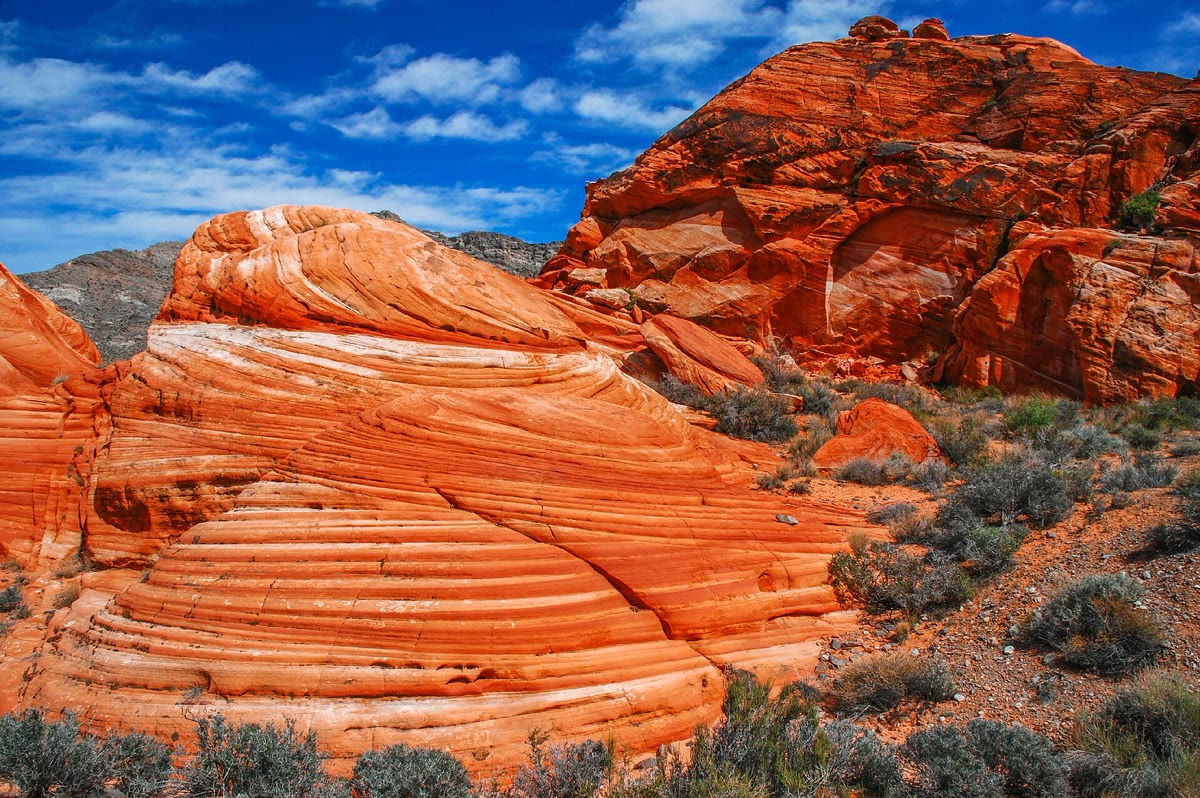
\includegraphics[height=3.6cm]{images/book3/b1-cross-bedding-aztec.jpg}};
\end{tikzpicture}

{\small À gauche~: la géométrie des \omterm{def:b1:clastic-sediments:bedform}{formes de fond} grimpantes (schématique, angles exagérés).
Les creux parcourent des trajectoires droites inclinées de l'angle de grimpage $\theta$
(traits épais)~; entre deux d'entre elles les parties inférieures des feuillets frontaux sont
préservées, en ensembles d'épaisseur $T = L\sin\theta$. À droite~: \omterm{def:b1:clastic-sediments:cross-bedding}{stratification entrecroisée} dans le
grès d'Aztec, Muddy Mountains, Nevada~: ensembles inclinés de laminae, chacun coupé
en haut par la surface d'érosion à la base du suivant. Photographie Chip Carroon,
Bureau of Land Management, CC~BY-SA~2.0, via Wikimedia Commons.}
\label{fig:b1:clastic-sediments:climb}
\end{omfigure}
% ledger: southard:climb, commons:aztec-crossbed

\emph{Les \omterm{def:b1:clastic-sediments:cross-bedding}{paléocourants}.} Les \omterm{def:b1:geological-maps:attitude}{sens du pendage} des strates entrecroisées mesurés sur un \omterm{def:b1:geological-maps:geological-map}{affleurement}
se dispersent autour de la direction moyenne du courant, parce que les faces aval des
\omterm{def:b1:clastic-sediments:bedform}{dunes} et des \omterm{def:b1:clastic-sediments:bedform}{rides} sont courbes et que les courants eux-mêmes divaguent. Leur moyenne se
prend comme une moyenne vectorielle, non arithmétique, pour la raison montrée à la
\cref{prop:b1:field-lab-methods-1:vector-mean}~: les \omterm{def:b1:spherical-astronomy:horizontal}{azimuts} sont des angles sur un
cercle, et 350 et 010 ont pour moyenne 000, non 180.

\begin{proposition}[Moyenne d'azimuts]\label{prop:b1:clastic-sediments:azimuths}
Soient $\alpha_1, \ldots, \alpha_N$ des \omterm{def:b1:spherical-astronomy:horizontal}{azimuts}, mesurés dans le sens horaire à partir du nord.
Leur moyenne vectorielle $\bar\alpha$ et leur longueur résultante moyenne $\bar R$ sont
données par
\[
  S = \sum_{i=1}^N \sin\alpha_i, \quad C = \sum_{i=1}^N \cos\alpha_i, \quad
  \bar\alpha = \operatorname{atan2}(S, C), \quad \bar R = \frac{\sqrt{S^2 + C^2}}{N},
\]
où $\operatorname{atan2}(S, C)$ est l'angle dont le sinus et le cosinus sont
proportionnels à $S$ et à $C$, pris entre \ang{0} et \ang{360}. $\bar R$ est compris
entre 0 et 1, et vaut 1 seulement si tous les \omterm{def:b1:spherical-astronomy:horizontal}{azimuts} sont égaux.
\end{proposition}

\begin{proof}
Le vecteur unitaire d'\omterm{def:b1:spherical-astronomy:horizontal}{azimut} $\alpha$, avec l'est comme première coordonnée et le nord
comme seconde, est $(\sin\alpha, \cos\alpha)$. La somme des $N$ vecteurs unitaires est
$(S, C)$, et sa direction, la moyenne vectorielle
(\cref{def:b1:field-lab-methods-1:mean-orientation}), a pour \omterm{def:b1:spherical-astronomy:horizontal}{azimut} celui dont le
sinus et le cosinus sont $S/\sqrt{S^2+C^2}$ et $C/\sqrt{S^2+C^2}$. D'après l'inégalité
triangulaire la longueur d'une somme de $N$ vecteurs unitaires est au plus $N$, avec égalité
seulement quand ils pointent tous dans le même sens.
\end{proof}

\begin{method}[Un paléocourant à partir de la stratification entrecroisée]\label{met:b1:clastic-sediments:palaeocurrent}
\begin{enumerate}
  \item Sur chaque ensemble, mesurer le \omterm{def:b1:geological-maps:attitude}{sens du pendage} des feuillets frontaux, en choisissant
        des surfaces qui montrent leur vrai \omterm{def:b1:geological-maps:attitude}{pendage} (ou mesurer direction et \omterm{def:b1:geological-maps:attitude}{pendage}).
  \item Mesurer l'\omterm{def:b1:geological-maps:attitude}{attitude} de la stratification principale~; si elle est inclinée de plus de
        quelques degrés, ramener chaque feuillet frontal à l'horizontale autour de la direction
        de la stratification (une rotation faite avec la projection stéréographique du volume de troisième année).
  \item Calculer la moyenne vectorielle $\bar\alpha$ et $\bar R$ des sens de \omterm{def:b1:geological-maps:attitude}{pendage}
        corrigés (\cref{prop:b1:clastic-sediments:azimuths}).
  \item Tracer les lectures en diagramme en rose, un histogramme circulaire d'\omterm{def:b1:spherical-astronomy:horizontal}{azimuts},
        pour voir si elles forment un groupe ou deux~: des courants de marée qui s'inversent
        construisent des ensembles qui plongent en sens opposés, en \omterm{def:b1:clastic-sediments:cross-bedding}{stratification
        entrecroisée} en arêtes de poisson, et une moyenne unique n'a alors aucun sens.
\end{enumerate}
\end{method}
% ledger: og:sorting-environments

\emph{Autres structures.} Plusieurs autres structures enregistrent les conditions de
dépôt et le sens du haut des bancs. Un \omterm{def:b1:clastic-sediments:turbidite}{banc granoclassé} s'affine vers le haut, du grossier à
sa base au fin à son sommet, à mesure que les grains se déposent depuis un courant qui décroît, les
plus grossiers d'abord (\cref{def:b1:clastic-sediments:turbidite}). Les fentes de
dessiccation, polygones de fentes de retrait remplies par la couche suivante, se forment là où la boue sèche à l'air,
comme sur les estrans et les plaines d'inondation. Les affouillements creusés par le courant dans la boue
en dessous, et remplis par le sable au-dessus, sont préservés comme moulages à la base du
banc de grès, et leurs formes indiquent le sens où le courant est allé.
% ledger: og:sorting-environments

\section{Faciès, rivières et deltas}\label{sec:b1:clastic-sediments:rivers-deltas}

La taille des grains, le \omterm{def:b1:clastic-sediments:sorting}{classement}, les structures, les fossiles et la composition font ensemble le
caractère d'une roche sédimentaire, et les géologues emploient un mot pour ce
caractère.

\begin{definition}[Faciès sédimentaire, milieu de dépôt]\label{def:b1:clastic-sediments:facies}
Un \emph{faciès sédimentaire}\index{facies sedimentaire@faciès sédimentaire} est un corps de roche sédimentaire
distingué des autres par sa lithologie, la taille des grains, ses structures sédimentaires
et ses fossiles, tous reflets des conditions dans lesquelles il s'est
formé. Le \emph{milieu de dépôt}\index{milieu de depot@milieu de dépôt} est
le lieu, avec ses conditions physiques, chimiques et biologiques, où un
sédiment est déposé~: un chenal de rivière, une plaine d'inondation, une plage, la pente d'un
delta, le fond marin profond.
\end{definition}
% ledger: og:sorting-environments

Un faciès est une description, un milieu une interprétation, et plusieurs
milieux peuvent faire le même faciès~: du sable à \omterm{def:b1:clastic-sediments:bedform}{rides} est déposé dans les rivières, sur les
estrans et sur le fond marin profond. L'interprétation repose donc sur des
associations de faciès et sur l'ordre dans lequel ils sont empilés, qui suivent
le déplacement des milieux dans l'espace~: les lois générales de cet empilement,
et les modèles standards de chaque milieu, sont le sujet du volume de troisième année. Ce
chapitre décrit les principaux milieux clastiques et les successions verticales
qui les identifient.

\emph{Rivières en tresses et à méandres.} Les rivières sont de deux styles principaux. Une rivière
en tresses s'écoule en de nombreux chenaux qui se divisent et se rejoignent autour de barres de gravier et de
sable~; les rivières en tresses portent des charges grossières près de leurs sources, sous les montagnes ou
devant les glaciers, et leurs dépôts sont des nappes de gravier et de sable grossier
à \omterm{def:b1:clastic-sediments:cross-bedding}{stratification entrecroisée}, avec peu de boue. Une rivière à méandres s'écoule dans un seul chenal
sinueux. L'eau la plus rapide court le long de l'extérieur de chaque courbe, où
elle érode la rive concave~; à l'intérieur, où l'eau est la plus lente, du sable est déposé
sur la barre de méandre. Le méandre migre ainsi latéralement, érodant d'un côté
et construisant de l'autre~; la plaine d'inondation au-delà des berges ne reçoit que la
boue des crues.
% ledger: og:rivers

La succession de la barre de méandre découle des \omterm{def:b1:clastic-sediments:bedform}{formes de fond}. Au pied de la
barre, dans l'eau la plus profonde et la plus rapide, le courant laisse les grains les plus grossiers
et construit des \omterm{def:b1:clastic-sediments:bedform}{dunes}~; en montant la barre en pente douce l'eau devient moins profonde et plus
lente, le sable plus fin et les \omterm{def:b1:clastic-sediments:bedform}{dunes} cèdent la place aux \omterm{def:b1:clastic-sediments:bedform}{rides}
(\cref{sec:b1:clastic-sediments:bedforms})~; au sommet, la barre passe à
la plaine d'inondation. À mesure que le méandre migre, chacune de ces zones se déplace sur celle
du dessous, et un forage à travers le dépôt les rencontre empilées~: une succession
à granoclassement normal d'une surface d'érosion à la boue, une pour chaque passage d'un chenal,
dont l'épaisseur est à peu près la profondeur du chenal qui l'a faite.

\emph{Les deltas.} Là où une rivière entre dans une étendue d'eau stagnante, son courant
s'étale et ralentit, et sa charge est déposée~: la charge grossière près de l'embouchure, la
charge fine plus loin. Un delta grandit vers l'avant, ou prograde, tant que la
rivière apporte plus de sédiments que les vagues et les marées n'en peuvent emporter. Ce que les
vagues et les marées font de l'apport décide de sa forme.

\begin{definition}[Deltas dominés par la rivière, par les vagues et par les marées]\label{def:b1:clastic-sediments:delta}
Un delta est \emph{dominé par la rivière}\index{delta domine par la riviere@delta dominé par la rivière} quand l'apport de la rivière
submerge les vagues et les marées, et que ses chenaux distributaires, confinés par
leurs propres levées, construisent de longs doigts de sable dans la mer~; il est
\emph{dominé par les vagues}\index{delta domine par les vagues@delta dominé par les vagues} quand les vagues remanient le sable
apporté aux embouchures en plages et en cordons littoraux le long d'une côte lisse et
arquée~; il est \emph{dominé par les marées}\index{delta domine par les marees@delta dominé par les marées} quand les
courants de marée, entrant et sortant des embouchures, façonnent son sable en barres et en crêtes
parallèles à l'écoulement, séparées par des chenaux en entonnoir.
\end{definition}
% ledger: og:deltas

\begin{omfigure}
\begin{tikzpicture}[font=\footnotesize, >={Stealth[length=4pt]}]
% meander in plan view (schematic) and the fining-upward log of a point bar
\begin{scope}[yscale=0.8]
  \fill[green!8] (-0.2,-0.4) rectangle (7.2,4.4);
  \draw[omSea!80!black, line width=9pt] plot[smooth, tension=0.7] coordinates {(0,3.6) (1.4,3.7) (2.6,2.8) (2.3,1.4) (3.2,0.5) (4.6,0.8) (5.0,2.2) (5.6,3.4) (7.0,3.5)};
  \draw[omSea!45, line width=7pt] plot[smooth, tension=0.7] coordinates {(0,3.6) (1.4,3.7) (2.6,2.8) (2.3,1.4) (3.2,0.5) (4.6,0.8) (5.0,2.2) (5.6,3.4) (7.0,3.5)};
  % point bars (inside of bends) with scroll lines
  \foreach \r in {0.25,0.45,0.65} {\draw[brown!60!black, densely dotted] (3.45,1.15) ++(200:\r) arc[start angle=200, end angle=340, radius=\r];}
  \fill[brown!25, opacity=0.8] (3.45,1.25) ellipse[x radius=0.55, y radius=0.35];
  \node[align=center] at (3.8,2.05) {barre de méandre\\ (dépôt)};
  \fill[brown!25, opacity=0.8] (1.75,2.75) ellipse[x radius=0.4, y radius=0.45];
  \node[align=center] at (1.2,1.95) {barre de\\ méandre};
  \draw[red!60!black, thick] (2.9,0.2) .. controls (3.3,0.0) and (4.3,0.15) .. (4.85,0.6);
  \node[red!60!black, anchor=north] at (4.0,0.0) {rive concave (érosion)};
  \draw[->, black!70] (5.9,3.0) -- (6.8,3.15) node[midway, below] {écoulement};
  \node[anchor=north west, black!60, align=left] at (5.2,1.3) {plaine\\ d'inondation};
  \node[font=\footnotesize] at (3.5,-0.85) {(a) un méandre, en plan};
\end{scope}
\begin{scope}[xshift=9.2cm, yshift=-0.3cm, yscale=0.8]
  % log: x width = grain size; y = height
  \draw[lith shale] (0,3.6) rectangle (0.8,4.6);
  \draw[lith sandstone] (0,2.6) rectangle (1.2,3.6);
  \draw[lith sandstone] (0,0.6) rectangle (1.7,2.6);
  \draw[lith conglomerate] (0,0) rectangle (2.2,0.6);
  \draw[very thick, red!60!black] (0,0) -- (2.2,0);
  % cross-bed symbols
  \foreach \y in {0.9,1.5,2.1} {\draw[black!70] (0.3,\y) .. controls (0.6,\y+0.05) and (0.9,\y+0.25) .. (1.2,\y+0.4);}
  \foreach \x in {0.2,0.5,0.8} {\draw[black!70] (\x,3.0) -- ++(0.12,0.1) -- ++(0.12,-0.1);}
  \node[anchor=west, align=left] at (2.4,4.1) {boue de plaine d'inondation,\\ racines, fentes de dessiccation};
  \node[anchor=west, align=left] at (2.4,3.1) {sable fin, lamination\\ oblique de rides};
  \node[anchor=west, align=left] at (2.4,1.6) {sable moyen à grossier,\\ stratification entrecroisée\\ de dunes};
  \node[anchor=west, align=left] at (2.4,0.3) {dépôt résiduel de gravier\\ sur une surface d'érosion};
  \draw[->] (-0.35,0) -- (-0.35,4.6) node[above] {haut};
  \draw[<->, black!60] (-0.7,0) -- node[above, rotate=90, font=\scriptsize] {profondeur du chenal} (-0.7,3.6);
  \node[font=\footnotesize] at (1.8,-0.5) {(b) succession d'une barre de méandre};
\end{scope}
\end{tikzpicture}

{\small (a)~Une rivière à méandres (schématique)~: le courant érode la berge extérieure de
chaque courbe et dépose du sable sur la barre de méandre à l'intérieur~; les lignes courbes de
sillons sont les positions successives de la barre. (b)~La succession laissée par une barre de méandre
en migration, la largeur de chaque couche proportionnelle à la taille de ses grains (schématique). Elle
s'affine vers le haut, et son épaisseur enregistre la profondeur du chenal.}
\label{fig:b1:clastic-sediments:point-bar}
\end{omfigure}
% ledger: og:rivers, southard:phase-diagram

Les trois pôles sont les sommets d'un triangle dans lequel tout delta peut être
placé selon la force relative des trois processus. Le delta en patte d'oiseau du
Mississippi, avec ses longs doigts dans le golfe du Mexique
(\cref{ch:b1:erosion-transport}), est le delta classique \omterm{def:b1:clastic-sediments:delta}{dominé par la rivière}~; le
Nil, avec son arc lisse de plages, un \omterm{def:b1:clastic-sediments:delta}{dominé par les vagues}~; le delta du
Gange et du Brahmapoutre, le plus grand du monde, un \omterm{def:b1:clastic-sediments:delta}{dominé par les marées}.
% ledger: og:deltas

\begin{omfigure}
\begin{tikzpicture}[font=\footnotesize]
% delta classification triangle (schematic) and the Lena delta from Landsat
\begin{scope}[yscale=0.82]
  \coordinate (R) at (2.6,4.5); \coordinate (W) at (0,0); \coordinate (T) at (5.2,0);
  \fill[omDef!8] (R) -- (W) -- (T) -- cycle;
  \draw[thick] (R) -- (W) -- (T) -- cycle;
  \node[above, align=center] at (R) {\textbf{dominé par la rivière}\\ doigts allongés, levées};
  \node[below, align=center] at (W) {\textbf{dominé par les vagues}\\ cordons littoraux lisses};
  \node[below, align=center] at (T) {\textbf{dominé par les marées}\\ barres parallèles\\ à l'écoulement};
  \fill[omThm] (2.6,2.9) circle[radius=2pt] node[below=1pt] {Mississippi};
  \fill[omThm] (0.75,0.4) circle[radius=2pt] node[above right=0pt] {Nil};
  \fill[omThm] (4.4,0.4) circle[radius=2pt] node[above left=0pt, align=right] {Gange--\\ Brahmapoutre};
\end{scope}
\node[anchor=south west, inner sep=0] at (7.2,-0.9) {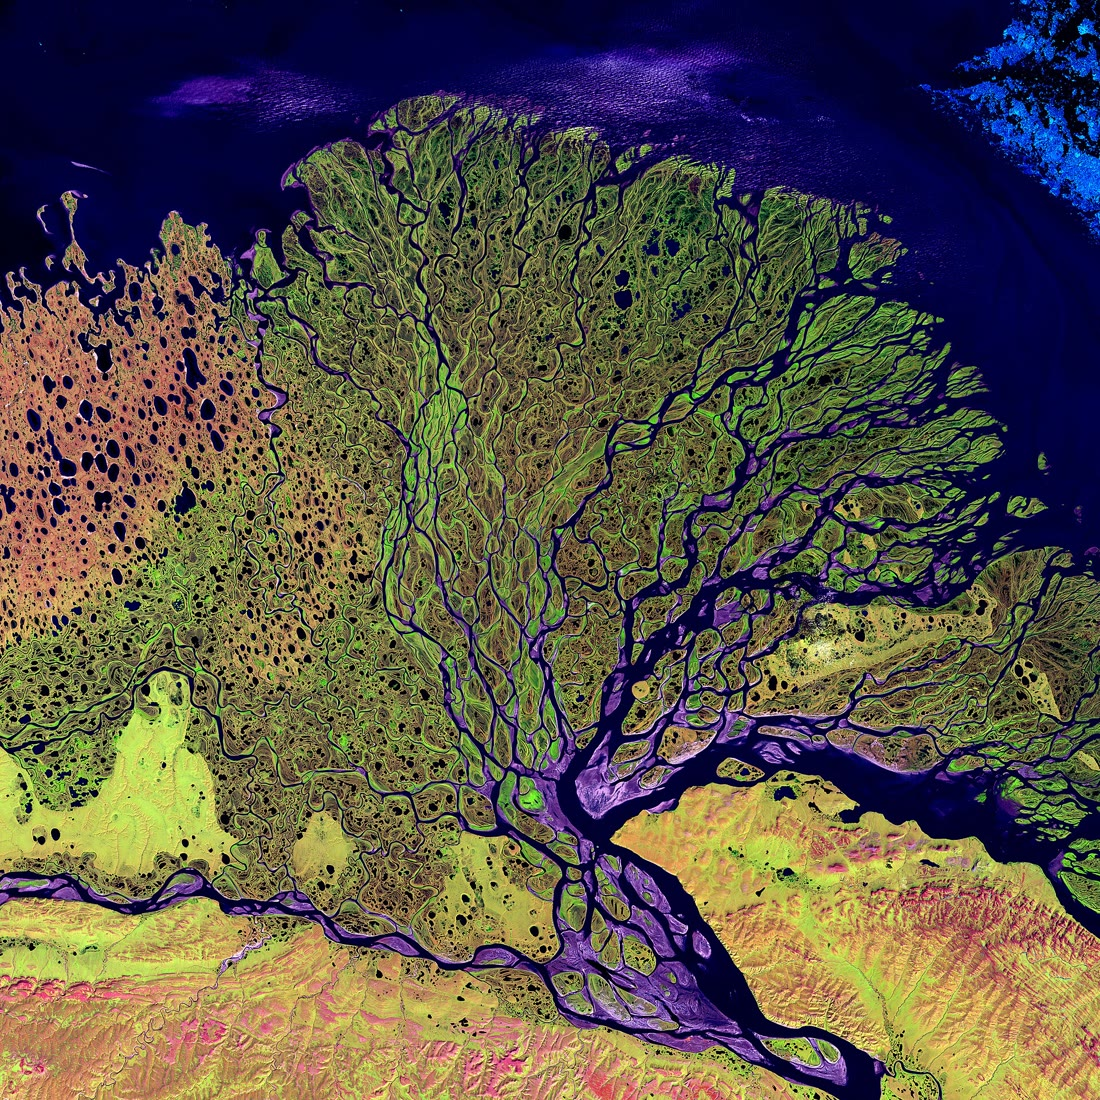
\includegraphics[height=5.2cm]{images/book3/b1-lena-delta.jpg}};
\end{tikzpicture}

{\small À gauche~: les trois pôles des deltas, d'après le processus qui les façonne
(schématique~; les positions des trois exemples sont indicatives). À droite~:
le delta de la Léna, en Sibérie, construit dans la mer des Laptev (en haut)~; le fleuve
entre par le bas à droite et se divise en centaines de distributaires. Image
en fausses couleurs Landsat~7 du 27~février 2000, U.S. Geological Survey, domaine public, via
Wikimedia Commons.}
\label{fig:b1:clastic-sediments:deltas}
\end{omfigure}
% ledger: og:deltas, commons:lena-delta

\emph{La succession à granocroissance.} Devant l'embouchure du fleuve, le
delta a un front en pente douce, le front de delta, qui passe vers le large au
prodelta, où seule la boue se dépose depuis la suspension. À mesure que le delta progresse, chacune
de ces zones avance sur celle qui est devant elle~: un forage sur la plaine
deltaïque rencontre, de bas en haut, les boues laminées du prodelta, puis des
alternances de silt et de sable du bas du front de delta, puis le sable à \omterm{def:b1:clastic-sediments:cross-bedding}{stratification entrecroisée}
des barres d'embouchure, coupé au sommet par les chenaux de la plaine deltaïque. La
succession se grossit vers le haut, l'inverse d'une barre de méandre, et son épaisseur est
à peu près la profondeur d'eau dans laquelle le delta s'est construit. Sa vitesse est liée à la
géométrie du front de delta.

\begin{proposition}[Progradation et accumulation]\label{prop:b1:clastic-sediments:progradation}
Soit un front de delta de pente constante $\alpha$ qui avance horizontalement à la vitesse
$v$ sans changer de forme, à niveau marin constant. Un point fixe sous le front
reçoit alors des sédiments à la vitesse verticale
\[
  a = v\,\tan\alpha,
\]
et la succession du front de delta d'épaisseur $h$ s'y accumule dans le temps
$h/(v\tan\alpha)$.
\end{proposition}

\begin{proof}
Dans le temps $\mathrm dt$ le front avance de $v\,\mathrm dt$. En un point
fixe sous la surface en pente, la surface s'élève de la différence de
hauteur entre deux points du front distants horizontalement de $v\,\mathrm dt$,
c'est-à-dire $v\,\mathrm dt\,\tan\alpha$, d'où la vitesse. Le front franchit
le point pendant que la surface s'élève de $h$, ce qui prend le temps $h/a$.
\end{proof}

Les fronts de delta sont en pente douce, donc $\tan\alpha$ est petit~: le front d'un delta
avance bien plus vite que les sédiments ne s'empilent en tout point sous lui
(\cref{exo:b1:clastic-sediments:12}).

\begin{inthelab}[Décrire une carotte]
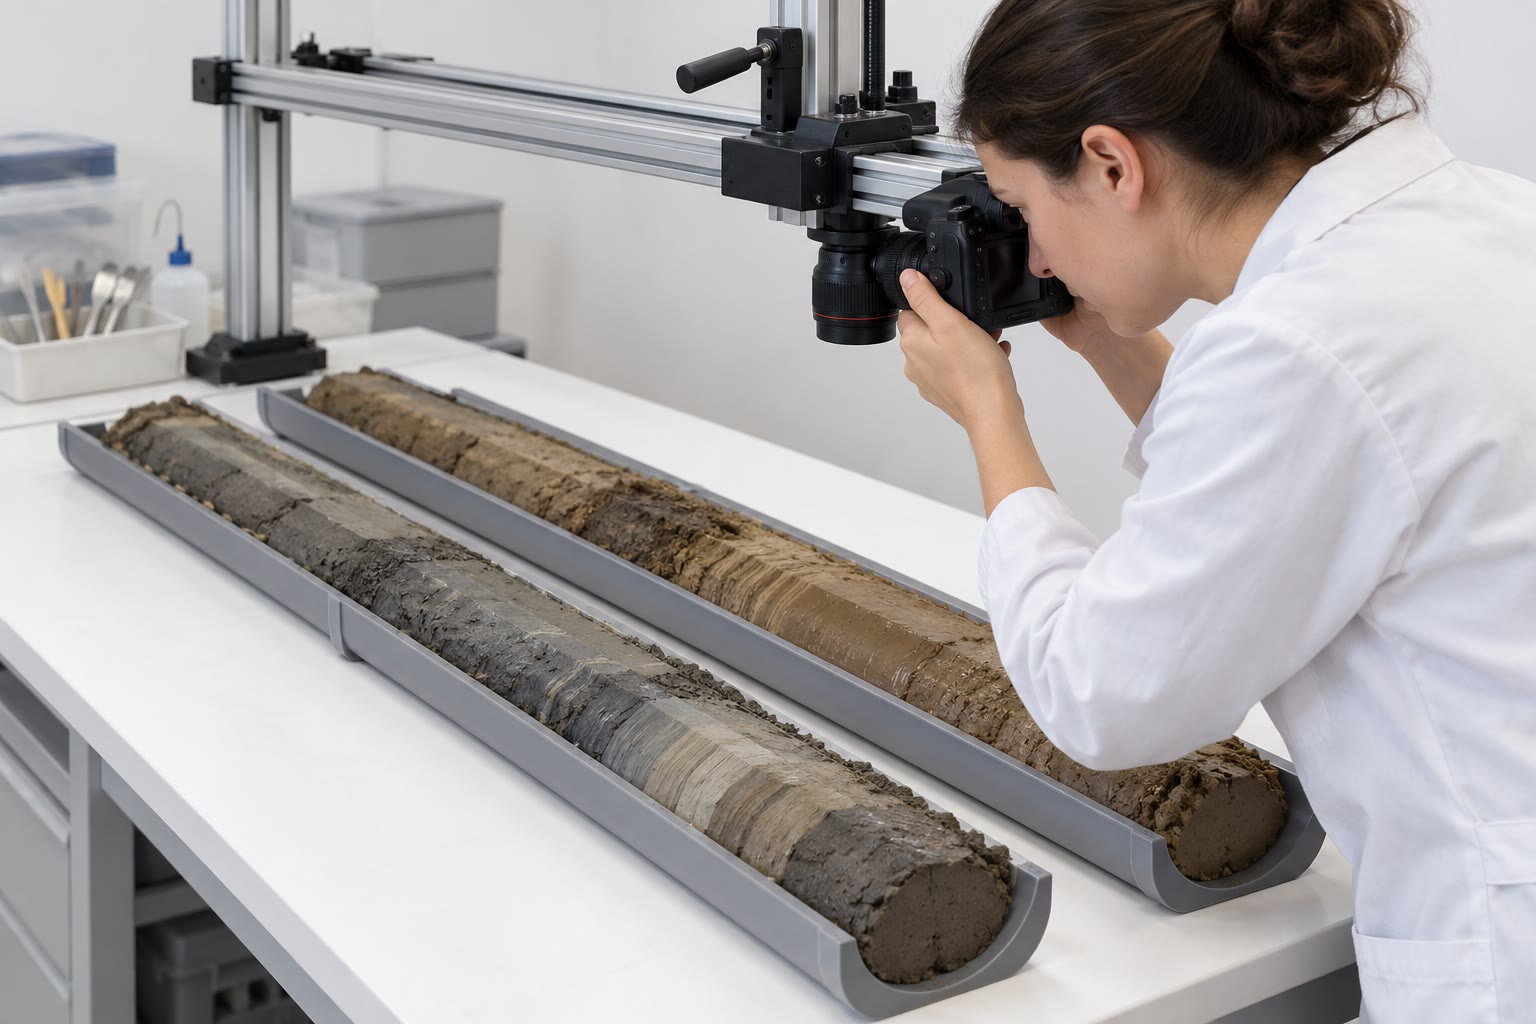
\includegraphics[width=0.3\linewidth]{images/book3/ai/b1-core-lab.jpg}\hfill
\begin{minipage}[b]{0.67\linewidth}
Les cylindres de sédiment ou de roche remontés par un forage sont rangés dans des bacs dans
l'ordre de la profondeur, fendus dans le sens de la longueur, et photographiés sous une lumière uniforme avant
qu'ils sèchent et changent de couleur. Le sédimentologue dessine alors un log de la carotte,
mètre par mètre~: la lithologie, la taille des grains de chaque banc (la largeur de la
colonne), les structures (\omterm{def:b1:clastic-sediments:cross-bedding}{stratification entrecroisée}, lamination, granoclassement, terriers), les
\omterm{def:b1:geological-maps:geological-map}{contacts}, nets ou graduels, la couleur et les fossiles. Des échantillons sont prélevés pour
l'analyse granulométrique et les \omterm{def:b1:field-lab-methods-1:thin-section}{lames minces}. Une carotte est une seule fenêtre étroite~: le
sens des strates entrecroisées est perdu à moins que la carotte ait été orientée, et
l'extension latérale des bancs doit venir d'autres forages.
\end{minipage}

\smallskip
{\small Une carotte étalée pour être photographiée dans un laboratoire de sédimentologie (illustration
IA).}
\end{inthelab}

\section{Rivage et plateau continental}\label{sec:b1:clastic-sediments:shoreline}

Le long de la côte entre les deltas, le sable apporté par les rivières est façonné par
les vagues et les marées. Une plage est du sable remanié par le jet de rive, la mince nappe d'eau
qui monte et descend sur elle après chaque déferlement de vague~: les grains sont déplacés sans cesse,
les fins sont emportés au large, et les sables de plage sont parmi les mieux
classés et les plus arrondis de tous les sédiments. Leurs laminae, déposées par le
jet de rive, plongent doucement vers le large. Sur de nombreuses côtes basses le sable forme des îles-barrières,
longs cordons de plage et de \omterm{def:b1:clastic-sediments:bedform}{dunes} éoliennes séparés du continent par
des lagunes, calmes et à grain fin, reliées à la mer par des passes
de marée.

Là où les marées sont fortes et les vagues faibles, la côte est bordée d'estrans,
couverts et découverts deux fois par jour. Ils passent du sable près de la ligne de basse mer,
où les courants sont les plus forts, à la boue près de la ligne de haute mer, où
l'eau étale laisse l'argile se déposer~; leurs dépôts montrent l'écoulement qui s'inverse en
\omterm{def:b1:clastic-sediments:cross-bedding}{stratification entrecroisée} en arêtes de poisson, l'assèchement dans les fentes de dessiccation, et l'alternance
de courant et d'eau étale dans de minces couches de boue drapant du sable à \omterm{def:b1:clastic-sediments:bedform}{rides}.

Au large, le plateau n'est balayé par les vagues que jusqu'à une profondeur qui croît avec la
taille des vagues. Au-dessus le sable est vanné et déplacé~; en dessous la boue se dépose,
sauf pendant les tempêtes, quand les plus grosses vagues atteignent plus profond et déposent des nappes de
sable à la douce lamination ondulée appelée \omterm{def:b1:clastic-sediments:cross-bedding}{stratification entrecroisée} en dôme.
Une succession de plateau alterne donc souvent boue de beau temps et sables de tempête, les
plus épais et les plus grossiers vers le rivage.
% ledger: og:sorting-environments, folk:maturity

\section{Les clastiques de mer profonde}\label{sec:b1:clastic-sediments:deep-sea}

Le sable et le gravier atteignent aussi les fonds des océans profonds, à des milliers de mètres
de profondeur et à des centaines de kilomètres de la terre, et ils y sont portés par des écoulements
que nul n'a vus en entier~: des courants denses chargés de sédiments descendant
la pente continentale sous l'eau claire de l'océan.

\begin{history}[Des câbles sur le fond marin, 1929]
Le 18~novembre 1929 un séisme de \omterm{def:b1:earthquake-source:mw}{magnitude de moment} 7.2 a frappé la pente continentale
au sud de Terre-Neuve, le long du bord sud des Grands Bancs. Un glissement
d'environ \qty{200}{km^3} de sédiments s'est mis en mouvement sur la pente, et un tsunami a tué 28
personnes sur la côte de Terre-Neuve. Douze câbles télégraphiques posés à travers le
fond marin se sont rompus, certains en plusieurs endroits. Ceux près de l'épicentre se sont rompus aussitôt~;
les autres, plus au sud et plus profonds, se sont rompus l'un après l'autre dans les heures
suivantes, dans l'ordre de la distance le long de la pente. En 1952 Bruce Heezen et Maurice Ewing,
étudiant les heures des ruptures, les expliquèrent~: le glissement s'était transformé en
\omterm{def:b1:clastic-sediments:turbidite}{courant de turbidité} qui avait couru le long de la pente et à travers la plaine abyssale sur
plus de 480 milles, rompant chaque câble à son passage. À partir des heures et des
distances ils estimèrent sa vitesse à environ 50 nœuds sur le haut glacis continental,
où la pente est d'environ \qty{0.5}{\percent}, et encore 12 nœuds au
dernier câble, à environ 400 milles de son origine. En ralentissant, soutinrent-ils, il avait dû
déposer un \omterm{def:b1:clastic-sediments:turbidite}{banc granoclassé} sur la plaine, de plus en plus fin vers le haut.
\end{history}
% ledger: nrcan:grand-banks, he52:grand-banks

Cinquante nœuds font \qty{25.7}{m.s^{-1}}, plus de \qty{90}{km.h^{-1}}, la vitesse d'une
voiture sur une route nationale~; 12 nœuds font \qty{6.2}{m.s^{-1}}~; et 480 milles font environ
\qty{770}{km}. Les ruptures ont aussi donné les premières vitesses mesurées d'un écoulement qui
n'avait été inféré qu'à partir de ses dépôts et d'expériences en cuve.
% ledger: he52:grand-banks

\begin{definition}[Courant de turbidité, turbidite, banc granoclassé]\label{def:b1:clastic-sediments:turbidite}
Un \emph{courant de turbidité}\index{courant de turbidite@courant de turbidité} est un courant d'eau rendu
plus dense que l'eau qui l'entoure par les sédiments qu'il tient en suspension, qui
s'écoule le long d'une pente sous cette eau, ses grains maintenus en suspension par la
turbulence que crée son propre mouvement. Une \emph{turbidite}\index{turbidite} est
le dépôt d'un courant de turbidité. Un \emph{banc granoclassé}\index{banc granoclasse@banc granoclassé} est un
banc dont la taille des grains décroît de sa base à son sommet.
\end{definition}
% ledger: og:sorting-environments, he52:grand-banks

Un \omterm{def:b1:clastic-sediments:turbidite}{courant de turbidité} s'entraîne lui-même~: il court parce que sa suspension est lourde, et
il garde sa suspension parce qu'il court. Sur une pente raide il peut ramasser davantage de
sédiment du fond, devenir plus dense et accélérer~; sur la pente douce de la
plaine abyssale il ralentit, laisse sa charge et meurt.

\begin{proposition}[Vitesse d'un courant de turbidité]\label{prop:b1:clastic-sediments:turbidity}
Un \omterm{def:b1:clastic-sediments:turbidite}{courant de turbidité} d'épaisseur $h$ et de masse volumique $\rho + \Delta\rho$ s'écoule
de façon permanente le long d'une pente $S$ sous de l'eau de masse volumique $\rho$. Si la résistance
du fond et de l'eau au-dessus est $\tau = \rho\,C_f\,U^2$ par unité d'aire, $C_f$
étant un coefficient de frottement sans dimension, sa vitesse moyenne est
\[
  U = \sqrt{\frac{\Delta\rho}{\rho}\,\frac{g\,h\,S}{C_f}} .
\]
\end{proposition}

\begin{proof}
L'argument est celui du produit profondeur--pente
(\cref{prop:b1:erosion-transport:depth-slope}), le poids étant remplacé par
le poids en excès. Une colonne du courant d'aire unité pèse $(\rho +
\Delta\rho) g h$, et l'eau qu'elle déplace $\rho g h$~: dans l'eau
environnante, seul l'excès $\Delta\rho\,g\,h$ le tire le long de la pente, avec la
composante $\Delta\rho\,g\,h\,S$ le long d'elle. En régime permanent cela équilibre la
résistance $\rho C_f U^2$, d'où $U^2 = (\Delta\rho/\rho)\,g\,h\,S/C_f$.
\end{proof}

La loi de résistance $\tau = \rho C_f U^2$, quadratique en la vitesse, est celle des
écoulements turbulents en hydraulique (les livres de physique), et $C_f$ se trouve par
l'expérience. La formule néglige l'eau que le courant mélange à lui-même
par sa surface supérieure, qui le dilue et le ralentit. Elle montre le rôle
des trois facteurs~: un courant deux fois plus épais, ou deux fois plus dense, ou sur une pente
deux fois plus raide, court $\sqrt 2$ fois plus vite. Une suspension contenant la
fraction $c$ de son volume sous forme de grains de quartz a $\Delta\rho/\rho = 1.65\,c$
(\cref{sec:b1:erosion-transport:settling}), petit sauf si l'écoulement est très
concentré~; c'est là qu'un \omterm{def:b1:clastic-sediments:turbidite}{courant de turbidité} diffère d'une rivière, dans laquelle
tout le poids de l'eau, non un petit excès, entraîne l'écoulement. Pour courir aux 50 nœuds de 1929 sur une pente d'un demi pour cent,
un \omterm{def:b1:clastic-sediments:turbidite}{courant de turbidité} a besoin d'un grand produit de l'épaisseur par l'excès de densité
(\cref{exo:b1:clastic-sediments:11}).

\emph{La séquence de Bouma.} En 1962 Arnold Bouma a décrit l'ordre interne des
bancs de grès des anciennes successions de mer profonde en cinq divisions, notées
de la base vers le haut. A~: sable massif ou granoclassé, souvent sur une base érosive~; B~: sable
à lamination parallèle~; C~: sable fin à lamination oblique de \omterm{def:b1:clastic-sediments:bedform}{rides}, souvent
convoluté~; D~: silt laminé passant à la boue~; E~: boue. L'ordre est lu comme
l'enregistrement d'un seul courant qui décroît passant sur un point~: en ralentissant, il laisse
d'abord ses grains les plus grossiers en masse, puis construit un fond plat supérieur, puis
des \omterm{def:b1:clastic-sediments:bedform}{rides}, puis laisse le silt et l'argile se déposer. Les séquences complètes sont rares~: les
divisions supérieures sont souvent érodées par le courant suivant, et loin de la source,
là où le courant est faible, les inférieures manquent.
% ledger: og:sorting-environments, shanmugam:bouma

\begin{omfigure}
\begin{tikzpicture}[font=\footnotesize]
% Bouma sequence: log (schematic) and a labelled photograph
\begin{scope}
  \draw[lith shale] (0,4.0) rectangle (0.7,4.8);
  \draw[lith shale] (0,3.3) rectangle (0.9,4.0);
  \draw[lith sandstone] (0,2.2) rectangle (1.3,3.3);
  \draw[lith sandstone] (0,1.2) rectangle (1.6,2.2);
  \draw[lith sandstone] (0,0) rectangle (2.0,1.2);
  \draw[very thick, red!60!black] (0,0) .. controls (0.6,-0.12) and (1.4,0.1) .. (2.0,0);
  \foreach \y in {1.4,1.6,1.8,2.0} {\draw[black!70] (0.1,\y) -- (1.5,\y);}
  \foreach \x in {0.15,0.5,0.85} {\draw[black!70] (\x,2.55) .. controls (\x+0.12,2.75) .. (\x+0.3,2.6);}
  \foreach \y in {3.45,3.6,3.75,3.9} {\draw[black!60] (0.1,\y) -- (0.8,\y);}
  \foreach \x/\y in {0.4/0.3, 0.9/0.5, 1.4/0.25, 0.6/0.8, 1.2/0.9} {\fill[black!60] (\x,\y) circle[radius=0.06];}
  \node[anchor=west] at (2.2,4.4) {E \quad boue};
  \node[anchor=west, align=left] at (2.2,3.75) {D \quad silt laminé passant\\ \phantom{D \quad}à la boue};
  \node[anchor=west, align=left] at (2.2,2.65) {C \quad lamination oblique\\ \phantom{C \quad}de rides};
  \node[anchor=west] at (2.2,1.7) {B \quad lamination parallèle};
  \node[anchor=west] at (2.2,0.6) {A \quad sable granoclassé};
  \node[anchor=west, red!60!black] at (2.2,-0.15) {base érosive, figures de semelle};
  \draw[->] (-0.3,0) -- (-0.3,4.8) node[above] {haut};
\end{scope}
\node[anchor=south west, inner sep=0] at (6.9,-0.3) {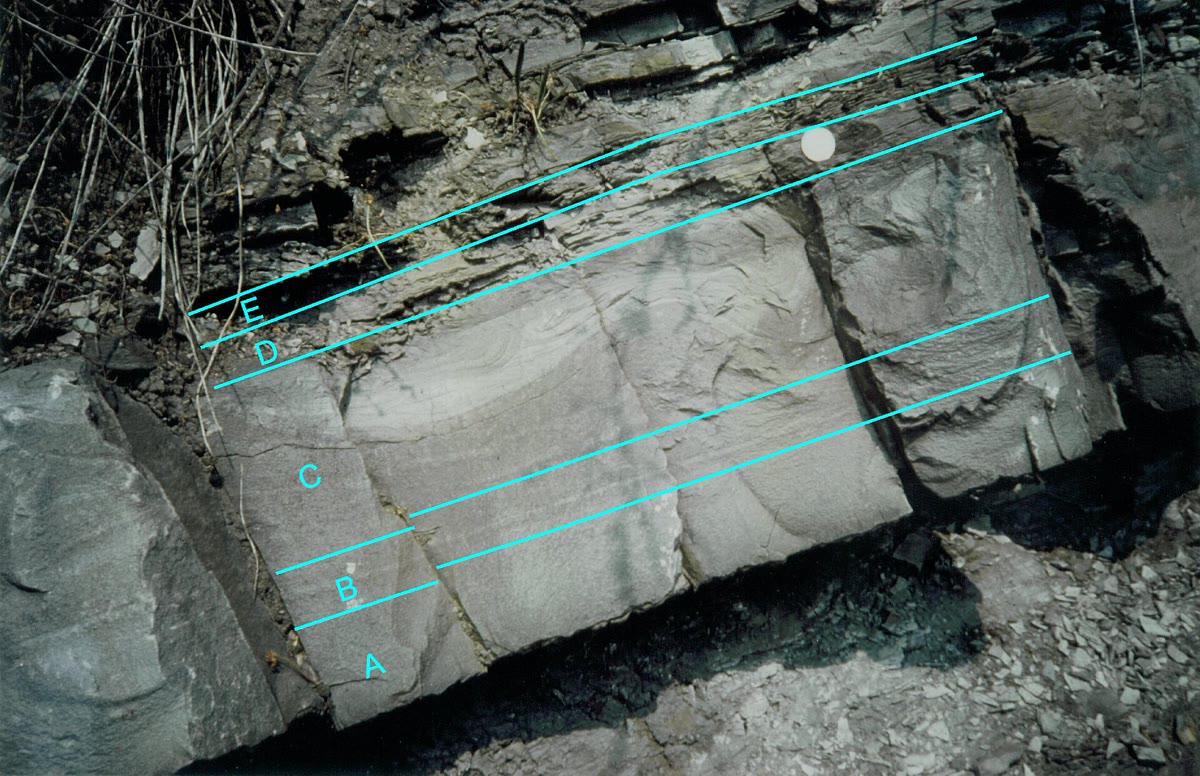
\includegraphics[height=5.2cm]{images/book3/b1-turbidite-bouma.jpg}};
\end{tikzpicture}

{\small À gauche~: les cinq divisions de la séquence de Bouma, la largeur de chacune
proportionnelle à la taille de ses grains (schématique). À droite~: un banc de \omterm{def:b1:clastic-sediments:turbidite}{turbidite} du Dévonien
supérieur à Becke-Oese, en Allemagne, avec les divisions A à E marquées par le
photographe~; la pièce donne l'échelle. Photographie Jo Weber, CC~BY-SA~3.0, via
Wikimedia Commons.}
\label{fig:b1:clastic-sediments:bouma}
\end{omfigure}
% ledger: og:sorting-environments, shanmugam:bouma, commons:bouma-becke-oese

La séquence de Bouma est devenue le modèle standard de la \omterm{def:b1:clastic-sediments:turbidite}{turbidite}, et des milliers
de grès anciens de mer profonde ont été interprétés avec elle. L'interprétation est
contestée~: des courants longeant la pente, des courants de marée profonds et des ondes internes
construisent aussi des sables à \omterm{def:b1:clastic-sediments:bedform}{rides} et laminés, et certains sédimentologues soutiennent
que de nombreux bancs lus comme des \omterm{def:b1:clastic-sediments:turbidite}{turbidites}, dont certains de ceux de la région type,
ont été déposés par d'autres écoulements. Peu de \omterm{def:b1:clastic-sediments:turbidite}{courants de turbidité} ont été observés dans
l'océan actuel, alors que les \omterm{def:b1:clastic-sediments:turbidite}{turbidites} anciennes se comptent par milliers.
% ledger: shanmugam:bouma

Toutes les clastiques de mer profonde ne sont pas des \omterm{def:b1:clastic-sediments:turbidite}{turbidites}. Les courants de contour, les courants lents et
profonds qui suivent les courbes de niveau de la pente continentale, remanient le sédiment
de la pente en dépôts lisses et allongés, les contourites. Et loin des
continents, là où ni les \omterm{def:b1:clastic-sediments:turbidite}{courants de turbidité} ni les courants de contour n'arrivent, le
fond marin ne reçoit que ce qui se dépose depuis l'eau au-dessus~: les coquilles du
plancton et les poussières éoliennes les plus fines, les sédiments pélagiques du chapitre
suivant (\cref{ch:b1:chemical-biogenic-sediments}).
% ledger: og:sorting-environments

\section{Exercices}

\begin{exercise}[$\star$]\label{exo:b1:clastic-sediments:1}
Convertir en unités phi les diamètres \qty{0.18}{mm}, \qty{0.75}{mm},
\qty{3}{mm}, \qty{0.012}{mm} et \qty{150}{mm}, à deux décimales, et nommer la
classe de chacun (\cref{tab:b1:clastic-sediments:classes}).
% ledger: folk:wentworth-classes
\end{exercise}

\begin{exercise}[$\star$]\label{exo:b1:clastic-sediments:2}
La courbe cumulative d'un sable de rivière donne $\varphi_5 = 0.62$, $\varphi_{16} =
1.05$, $\varphi_{50} = 1.71$, $\varphi_{84} = 2.43$ et $\varphi_{95} = 2.98$.
Calculer sa moyenne graphique, en unités phi et en millimètres, et son écart-type
graphique inclusif, et nommer sa taille et son \omterm{def:b1:clastic-sediments:sorting}{classement}.
% ledger: folk:graphic-measures, folk:sorting-classes
\end{exercise}

\begin{exercise}[$\star$]\label{exo:b1:clastic-sediments:3}
Des \omterm{def:b1:clastic-sediments:bedform}{rides} hautes de \qty{2}{cm} migrent à \qty{1}{cm} par minute sur un fond de sable de quartz
de porosité \num{0.4}. Avec la \cref{prop:b1:clastic-sediments:migration},
calculer le volume de \omterm{def:b1:erosion-transport:load}{charge de fond} par unité de largeur, en \si{m^2.s^{-1}}, et la masse
de quartz ($\qty{2650}{kg.m^{-3}}$) transportée par-dessus un mètre de crête en un jour.
% ledger: hom:quartz
\end{exercise}

\begin{exercise}[$\star$]\label{exo:b1:clastic-sediments:4}
Un nœud est un mille marin, \qty{1852}{m}, par heure. (a)~Convertir en mètres
par seconde les vitesses de 50 et 12 nœuds estimées pour le \omterm{def:b1:clastic-sediments:turbidite}{courant de turbidité} de
1929. (b)~Combien de temps un courant à 12 nœuds met-il pour couvrir \qty{100}{km}~?
(c)~Convertir 480 et 400 milles en kilomètres (un mille fait \qty{1.609}{km}).
% ledger: he52:grand-banks
\end{exercise}

\begin{exercise}[$\star\star$]\label{exo:b1:clastic-sediments:5}
(a)~Avec les percentiles d'une distribution normale donnés dans la démonstration de la
\cref{prop:b1:clastic-sediments:normal}, calculer l'écart-type
graphique $(\varphi_{84} - \varphi_{16})/2$ et l'estimation
$(\varphi_{95} - \varphi_5)/3.3$ pour une distribution normale d'écart-type
$\sigma$. (b)~Pourquoi les deux pourraient-ils différer pour un sédiment réel~? Quel
type de sédiment les fait différer le plus~?
\end{exercise}

\begin{exercise}[$\star\star$]\label{exo:b1:clastic-sediments:6}
Un dépôt de \omterm{def:b1:clastic-sediments:bedform}{rides} grimpantes montre des ensembles de \qty{1.5}{cm} d'épaisseur, mesurée
perpendiculairement à leurs limites, faits par des \omterm{def:b1:clastic-sediments:bedform}{rides} espacées de \qty{15}{cm}.
(a)~Calculer l'angle de grimpage. (b)~Si les \omterm{def:b1:clastic-sediments:bedform}{rides} se déplaçaient à
\qty{0.5}{cm} par minute, à quel rythme le fond s'est-il exhaussé, en centimètres par
heure~? (c)~Que dit un tel rythme de l'écoulement~?
% ledger: southard:climb
\end{exercise}

\begin{exercise}[$\star\star$]\label{exo:b1:clastic-sediments:7}
Six sens de \omterm{def:b1:geological-maps:attitude}{pendage} de strates entrecroisées, déjà corrigés de l'inclinaison des bancs,
valent 350, 020, 005, 340, 015 et 030. (a)~Calculer leur moyenne arithmétique. (b)~Calculer
leur moyenne vectorielle et $\bar R$. (c)~Expliquer la différence.
\end{exercise}

\begin{exercise}[$\star\star$]\label{exo:b1:clastic-sediments:8}
Trois grès sont examinés en \omterm{def:b1:field-lab-methods-1:thin-section}{lame mince}. A a \qty{12}{\percent} de
matrice argileuse et des grains anguleux de quartz, de \omterm{def:b1:rock-forming-minerals:groups}{feldspath} et de fragments de roche. B a
\qty{2}{\percent} d'argile, $\sigma_I = 0.40\,\varphi$ et des grains de quartz
d'arrondi \num{2.2} sur l'échelle de Folk. C n'a pas d'argile, $\sigma_I =
0.30\,\varphi$, des grains de quartz d'arrondi \num{3.6}, et \qty{98}{\percent}
de quartz. Nommer la \omterm{def:b1:clastic-sediments:maturity}{maturité texturale} de chacun, et proposer un \omterm{def:b1:clastic-sediments:facies}{milieu de
dépôt} pour chacun.
% ledger: folk:maturity
\end{exercise}

\begin{exercise}[$\star\star$]\label{exo:b1:clastic-sediments:9}
(a)~Calculer le nombre de Froude d'un écoulement profond de \qty{0.3}{m} à
\qty{1.5}{m.s^{-1}}, et d'une rivière profonde de \qty{2}{m} à \qty{1.0}{m.s^{-1}} ($g
= \qty{9.81}{m.s^{-2}}$). (b)~À quelle profondeur un écoulement à
\qty{1.5}{m.s^{-1}} atteindrait-il un nombre de Froude de 1, et quelle vitesse la rivière
profonde de \qty{2}{m} demanderait-elle~? (c)~Pourquoi les antidunes sont-elles courantes dans les nappes d'eau qui
s'écoulent d'une plage, et rares dans les grandes rivières~?
% ledger: southard:ripples-dunes
\end{exercise}

\begin{exercise}[$\star\star\star$]\label{exo:b1:clastic-sediments:10}
Une analyse granulométrique par tamisage d'un sable donne, en classes phi entières de $-1$ à
$5\,\varphi$~: 2, 8, 30, 40, 15 et 5 pour cent en poids. (a)~Par la méthode des
moments, calculer la moyenne et l'écart-type en unités phi, et nommer le
\omterm{def:b1:clastic-sediments:sorting}{classement}. (b)~Construire la courbe cumulative, lire $\varphi_5$, $\varphi_{16}$,
$\varphi_{50}$, $\varphi_{84}$ et $\varphi_{95}$ par interpolation linéaire, et
calculer $M_z$ et $\sigma_I$. (c)~Comparer.
% ledger: folk:graphic-measures, folk:sorting-classes
\end{exercise}

\begin{exercise}[$\star\star\star$]\label{exo:b1:clastic-sediments:11}
Prendre $C_f = 0.003$ dans la \cref{prop:b1:clastic-sediments:turbidity}. (a)~Un
\omterm{def:b1:clastic-sediments:turbidite}{courant de turbidité} épais de \qty{50}{m}, avec un excès de densité de
\qty{2}{\percent}, descend une pente de \num{0.005}~: calculer sa vitesse, en mètres
par seconde et en nœuds. (b)~Quel produit de l'épaisseur par l'excès relatif de densité
donnerait les 50 nœuds de 1929 sur la même pente~? (c)~Le même courant
qu'en (a) atteint une pente de \num{0.001}~: calculer sa nouvelle vitesse, si rien
d'autre ne change. Qu'advient-il de sa charge~?
% ledger: he52:grand-banks
\end{exercise}

\begin{exercise}[$\star\star\star$]\label{exo:b1:clastic-sediments:12}
Une rivière livre \qty{50}{Mt} de sédiments par an à son delta, dont
\qty{70}{\percent} sont déposés sur un front de delta large de \qty{100}{km} qui se construit
dans une eau profonde de \qty{30}{m}. Le dépôt a une masse volumique apparente de
\qty{2000}{kg.m^{-3}}. (a)~Quel volume ajoute-t-il chaque année~? (b)~Si ce volume
remplit toute la profondeur d'eau sur la largeur du front, à quelle vitesse le
front avance-t-il~? (c)~Avec une pente de front de delta de \ang{0.5}, à quel rythme
le sédiment s'empile-t-il en un point fixe sous le front, et en combien d'années
la succession à granocroissance s'y forme-t-elle~?
\end{exercise}

\section{Problème~: Lire une carotte d'un delta}

\begin{problem}[{Problème du week-end --- un forage à travers un ancien delta, des
tailles de grains au sens de ses rivières}]
\label{pb:b1:clastic-sediments:1}
% values: calc/ch21.py; the borehole, its beds, ages and readings are invented
Un forage traverse \qty{24}{m} de grès et d'argilites déposés par un
ancien delta. Le géologue décrit quatre unités, de la base vers le haut, et
analyse un échantillon de chacune.

\smallskip
\begin{center}\small
\begin{tabular}{@{}llccccc@{}}
\hline
unité (profondeur depuis la base) & description & $\varphi_5$ & $\varphi_{16}$ & $\varphi_{50}$ & $\varphi_{84}$ & $\varphi_{95}$ \\
\hline
1 (0--8 m) & argilite grise laminée & 4.2 & 5.0 & 6.6 & 8.4 & 9.6 \\
2 (8--16 m) & alternance de siltite et de grès & 1.9 & 2.4 & 3.4 & 4.6 & 5.5 \\
3 (16--21 m) & grès à \omterm{def:b1:clastic-sediments:cross-bedding}{stratification entrecroisée} & 0.9 & 1.25 & 1.8 & 2.35 & 2.7 \\
4 (21--24 m) & grès à cailloux, base érosive & $-1.8$ & $-0.8$ & 0.9 & 2.1 & 2.9 \\
\hline
\end{tabular}
\end{center}

\medskip
\noindent\textbf{Partie I --- Les tailles de grains.}
\begin{enumerate}
  \item Calculer la moyenne graphique $M_z$ de chaque unité, en unités phi et en
        millimètres.
  \item Calculer l'écart-type graphique inclusif $\sigma_I$ de chaque
        unité.
  \item Nommer la classe de taille de la moyenne et le \omterm{def:b1:clastic-sediments:sorting}{classement} de chaque unité.
  \item Quelle unité est la mieux classée~? Pourquoi une barre d'embouchure serait-elle mieux classée
        que les boues du prodelta~?
  \item En interpolant linéairement entre $\varphi_{50}$ et $\varphi_{84}$,
        estimer le pourcentage de particules de la taille de l'argile (plus fines que
        $8\,\varphi$) dans l'unité~1. Que dit-il des courants là où elle
        a été déposée~?
  \item Pourquoi la courbe cumulative de l'unité~4 est-elle si étalée, bien que ce soit un
        sable de chenal~?
\end{enumerate}

\medskip
\noindent\textbf{Partie II --- La succession.}
\begin{enumerate}[resume]
  \item Décrire comment la taille moyenne change de l'unité~1 à l'unité~3. La
        succession s'affine-t-elle ou se grossit-elle vers le haut~?
  \item Interpréter les unités 1, 2 et 3 comme des parties d'un delta. Quelle zone du delta
        se trouvait sur le site quand chacune a été déposée~?
  \item Que montre l'empilement des trois unités du déplacement du
        delta~?
  \item Dans quelle profondeur d'eau le delta s'est-il construit, au moins, et pourquoi~?
  \item L'unité~4 a une base érosive et est plus grossière que l'unité~3. L'interpréter.
  \item Une barre de méandre donnerait-elle la même succession~? Expliquer.
\end{enumerate}

\medskip
\noindent\textbf{Partie III --- À quelle vitesse le delta a-t-il avancé~?}
Deux minces bancs de cendres volcaniques, à la base de l'unité~1 et au sommet de
l'unité~2, sont datés~; ils sont distants de \num{4000}~ans.
\begin{enumerate}[resume]
  \item Calculer le taux moyen d'accumulation entre les deux cendres, en
        millimètres par an.
  \item Le front du delta avait une pente de \ang{0.5}. Avec la
        \cref{prop:b1:clastic-sediments:progradation}, calculer la vitesse à laquelle
        il a avancé, en mètres par an.
  \item De quelle distance le front a-t-il avancé pendant les \num{4000}~ans~?
  \item Combien de temps les 21 mètres des unités 1 à 3 ont-ils mis à s'accumuler sur le
        site, à ce rythme~?
  \item Pourquoi le taux d'accumulation dans un delta n'est-il pas le même partout au
        même moment~?
\end{enumerate}

\medskip
\noindent\textbf{Partie IV --- Où coulaient les rivières~?}
Sur le grès à \omterm{def:b1:clastic-sediments:cross-bedding}{stratification entrecroisée} de l'unité~3, exposé dans un \omterm{def:b1:geological-maps:geological-map}{affleurement} voisin où les
bancs sont horizontaux, douze sens de \omterm{def:b1:geological-maps:attitude}{pendage} de feuillets frontaux sont mesurés~: 352, 010, 025,
004, 338, 017, 031, 359, 012, 046, 006 et 344.
\begin{enumerate}[resume]
  \item Calculer la moyenne arithmétique des douze lectures. A-t-elle un sens~?
  \item Calculer les sommes $S$ et $C$ de la \cref{prop:b1:clastic-sediments:azimuths}.
  \item Calculer la longueur résultante moyenne $\bar R$. Les lectures sont-elles
        cohérentes~?
  \item Dans quelle direction générale le delta s'est-il construit, et où était la terre~?
  \item Pourquoi faut-il faire tourner les sens de \omterm{def:b1:geological-maps:attitude}{pendage} si les bancs sont inclinés, et
        autour de quel axe~?
  \item Un courant de marée aurait-il pu construire ces strates entrecroisées~? À quoi ressemblerait son
        diagramme en rose~?
  \item Au degré près, quel est l'\omterm{def:b1:spherical-astronomy:horizontal}{azimut} moyen du \omterm{def:b1:clastic-sediments:cross-bedding}{paléocourant} du grès
        à \omterm{def:b1:clastic-sediments:cross-bedding}{stratification entrecroisée} de l'unité~3~?
\end{enumerate}
\end{problem}
